%Formatvorgabe tobii ist toll beim Kellerpumpen
\documentclass[12pt,a4paper,oneside,bibliography=totocnumbered]{scrartcl}
\usepackage[ngerman]{babel}
\usepackage[utf8]{inputenc}
\usepackage[a4paper,left=4cm,right=2cm,top=3cm,bottom=2cm]{geometry}
\linespread{1.25}
\usepackage{fancyhdr}
\pagestyle{fancy}
\lhead{}
\rhead{\thepage}
\cfoot{}

%Hier sind die Daten der Seminararbeit
\newcommand{\MyAuthor}{René Spieker \& Tobias Wäschle (285524)}
\newcommand{\MyTitel}{SAP ERP - Rechnungswesen (FI, CO)}
\newcommand{\MyFirma}{Deutsche Telekom AG}
%\newcommand{\MyMatrikelNummer}{285524}
\newcommand{\MyBetreuer}{Dr.-Ing. Peter Steininger}
\newcommand{\MyKurs}{ERP-Systeme}
\newcommand{\MySemester}{4. Fachsemester}
\newcommand{\MyStudiengang}{Wirtschaftsinformatik}
\newcommand{\MyOrt}{Bonn}
\newcommand{\MyDatum}{\today}

%\usepackage{amsmath}

%\usepackage{amsfonts}
%\usepackage{amssymb}
%\usepackage{makeidx}
\usepackage{floatflt}
\usepackage{graphicx}
\usepackage{caption}
%Abkürzungsverzeichnis z.B. etc.\abk{etc.}{et cetera}
\usepackage{nomencl}
\usepackage{paralist}


\usepackage{mathptmx}
\usepackage{natbib}
\usepackage[hidelinks,
			pdfauthor={\MyAuthor},
			pdftitle={\MyTitel},
			pdfproducer={pdfLaTeX with hyperref},
			pdfcreator={pdfLaTeX}]{hyperref}

\author{\MyAuthor}
\title{\MyTitel}
\date{\MyDatum}
\makeindex
\begin{document}
%Diverse Verzechnisse
\newpage
\renewcommand{\thesection}{\Roman{section}}  % I, II, III, IV
\pagenumbering{Roman}
%\addsec{Fachwort- und Abkürzungsverzeichnis}
%\input{includes/fachwortverzeichnis}
%Titelseite
\begin{titlepage}
\raggedleft

\centering
\vfill
{\bfseries\Huge Seminararbeit}\\
\vfill
Titel der Seminararbeit\\[2ex]
{\bfseries\Large "`\MyTitel{}"'}\\[1ex]
{\bfseries\small -- \MySemester{} --}\\
\vfill
Verfasser: \MyAuthor{}\\
\vfill
\raggedright
\small
\MyOrt, den \MyDatum\\[2cm]
\begin{tabbing}
%Matrikelnummer: \= \MyMatrikelNummer{}\\
Studiengang: \= \MyStudiengang{}\\
Kurs: \> \MyKurs{}\\
Betreuer:  \> \MyBetreuer{}\\
\end{tabbing}
\end{titlepage}

%Weitere Seiten vor dem Hauptteil
%Sperrvermerk
%\newpage
%\thispagestyle{empty}
%\section*{Sperrvermerk}
Die vorliegende Seminararbeit mit dem Titel ``\MyTitel{}'' enthält unternehmensinterne Daten der Firma \MyFirma{} daher ist sie nur zur Vorlage bei der FOM sowie den Begutachtern der Arbeit bestimmt. Für die Öffentlichkeit und dritte Personen darf sie nicht zugänglich sein.
\\[3cm]
\begin{flushright}
\line(1,0){100} \hfill \line(1,0){150}\\
(Ort, Datum) \hfill \textbf{René Spieker}\\[1.5cm]
\line(1,0){100} \hfill \line(1,0){150}\\
(Ort, Datum) \hfill \textbf{Tobias Wäschle}\\
\end{flushright}

%Inhaltsverzeichnis
\newpage
%\thispagestyle{empty}
\tableofcontents



\addsec{Tabellenverzeichnis}
\renewcommand{\listtablename}{} 
\listoftables
\newpage
%\include{includes/tabellenverzeichnis}
\addsec{Abbildungsverzeichnis}
\renewcommand{\listfigurename}{} 
\listoffigures
%\include{includes/abbildungsverzeichnis}
\newpage

%%Abkürzungsverzeichnis z.B. etc.\abk{etc.}{et cetera}
 % Befehl umbenennen in abk
 \let\abk\nomenclature
 % Deutsche Überschrift
 \renewcommand{\nomname}{}
 % Punkte zw. Abkürzung und Erklärung
 \setlength{\nomlabelwidth}{.35\hsize}
 \renewcommand{\nomlabel}[1]{#1 \dotfill}
 % Zeilenabstände verkleinern
 \setlength{\nomitemsep}{-\parsep}
 \makenomenclature
 \addsec{Fachwort- und Abkürzungsverzeichnis}
\printnomenclature

%Hauptteil
\clearpage
\setcounter{section}{0}
\renewcommand{\thesection}{\arabic{section}} % 1, 2, 3, 4 ...
\pagenumbering{arabic}

\section{Einleitung}
\subsection{Einführung und Relevanz des Themas}
%Viele Unternehmen sehen sich neuen Aufgabenstellungen gegen{\"u}ber. Ursache sind die Internationalisierung, die h{\"a}ufigen Produktwechsel und der Zwang zu permanenter\\Veränderung. Der Anteil der Routineaufgaben nimmt stetig ab, w{\"a}hrend andererseits neuartige und komplexer werdende Aufgaben anstehen\footnote{Vgl. \cite{Fiedler2008}, S.~1}.
%Die Durchführung dieser Aufgaben wird in der Unternehmenspraxis zunehmend in Form von Projekten vollzogen.
%Dass komplexe, neuartige und interdisziplinäre Projekte nicht intuitiv ausgewählt und zum Ziel geführt werden können, dürfte heute jedem Unternehmer klar sein.
%
%In diesem Zusammenhang treten facettenreiche und h{\"o}chst unterschiedliche Problemfelder auf, denen von Seiten der Unternehmenspraxis wie auch der Betriebswirtschaftslehre begegnet werden muss. Um eine geeignete Projektauswahl und Implementierung der Unternehmensstrategien in diese Projekte zu gewährleisten, muss die Unternehmensf{\"u}hrung und die Projektleitung durch eine sinnvolle und methodisch gepr{\"a}gte Planung und Kontrolle der Projekte eines Unternehmens unterst{\"u}tzt werden\footnote{Vgl. \cite{Kunz2007}, S.~1} \footnote{Vgl. \cite{Urli&Terrien2010}}.

\subsection{Zielsetzung und Abgrenzung}
%Diese Arbeit beschäftigt sich mit theorieorientierten Ausprägungen und Beschreibungen des Projektcontrollings. Das Thema wird in sinnvollen Aufgabenbereichen strukturiert und näher analysiert. Es werden die Grundlagen des Projektmanagement vorausgesetzt und deshalb auf eine detaillierte Beschreibung der Methoden und Techniken der Organisation, Planung und Durchführung von Projektportfolios oder Projekten verzichtet.

\subsection{Vorgehen}
%Die Abbildung \ref{abb1} auf Seite \pageref{abb1} zeigt eine schematische Darstellung zum Aufbau der Arbeit.
%\begin{figure}[htbp]
%\begin{center}
%%\begin{floatingfigure}[r]{0.7\textwidth}
%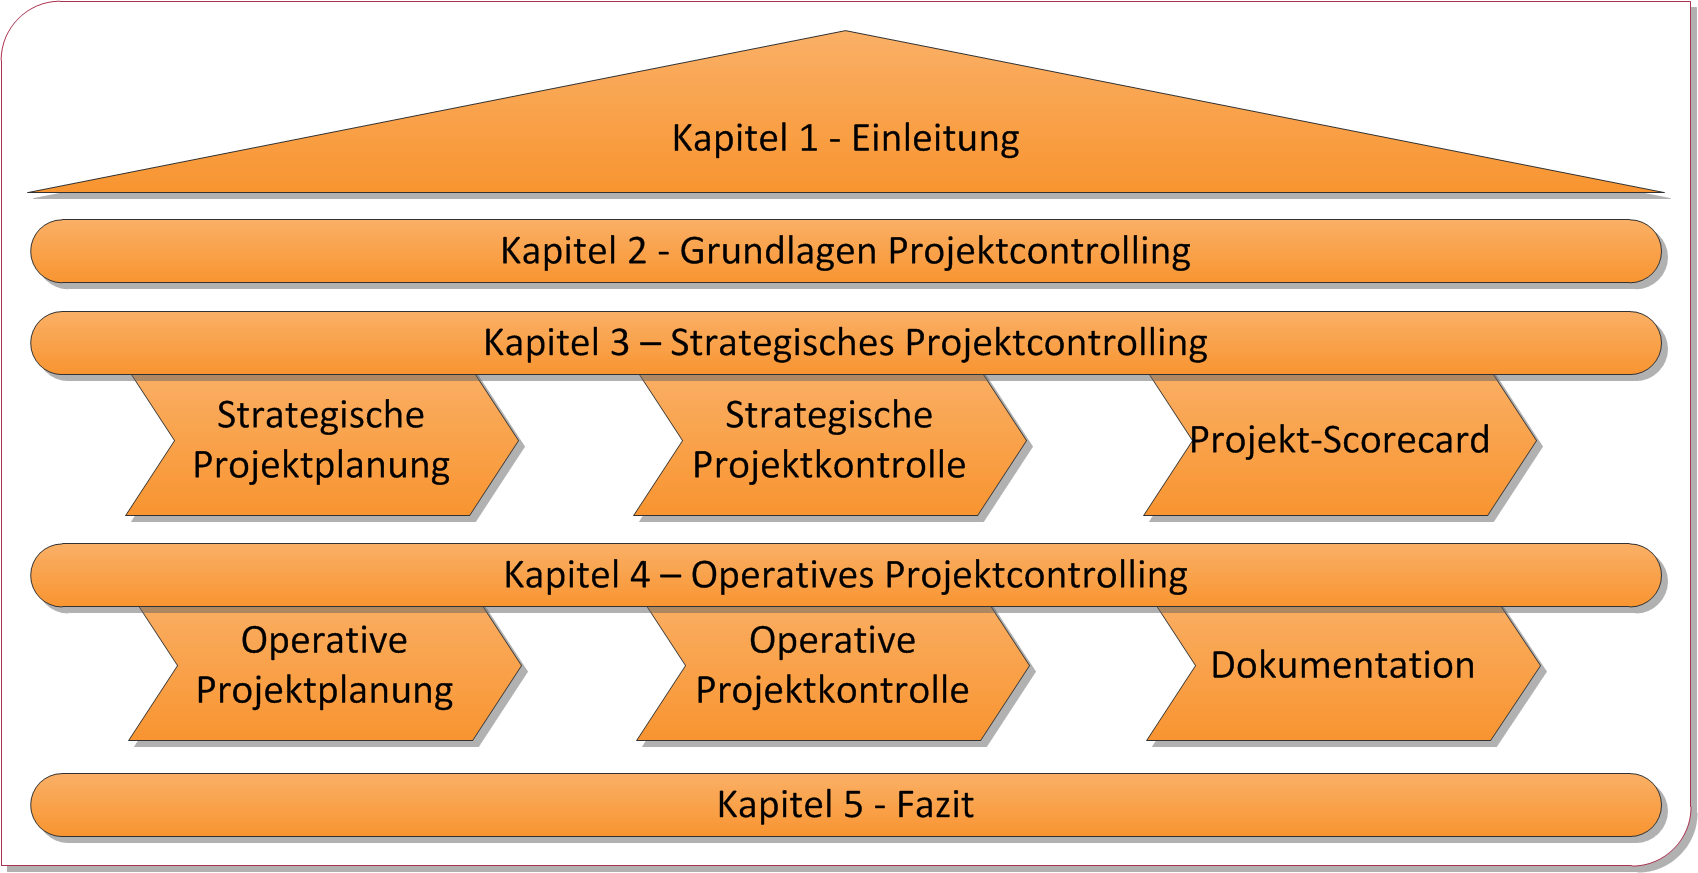
\includegraphics[width=0.8\textwidth]{Images/aufbau.png}
%\caption[Aufbau dieser Arbeit]{Aufbau dieser Arbeit}
%\label{abb1}
%\end{center}
%\end{figure}
%%\end{floatingfigure}
%\begin{compactitem}
%\item Kapitel 1 führt an das betrachtete Thema heran und definiert die Ziele dieser Arbeit.
%\item Kapitel 2 gibt einen Überblick über Projektcontrolling im Projektmanagement. Angesprochen werden die Ausprägungen, sowie die Aufgaben und Ziele des Projektcontrollings.
%\item Kapitel 3 behandelt das Projektcontrolling aus strategischer Sicht. Es wird die Auswahl und Priorisierung von Projekten in einem Projektportfolio erklärt, aber auch um den Einsatz der Project Scorecard für die Projektauswahl und Projektsteuerung.
%\item Kapitel 4 bildet den Schwerpunkt der Arbeit. Es beschreibt das operative Projektcontrolling und orientiert sich an den Lebenszyklusphasen eines Projektes. Die Sicht auf die Planung wird um die Aspekte der Steuerung und Kontrolle ergänzt.
%\item Kapitel 5 [...]tbd
%\end{compactitem}

\abk{DIN}{Deutsche Industrie-Norm}
\abk{Projekt}{casu quo (c. q.) nach  DIN 69901: zeitlich befristetes Vorhaben mit definiertem Anfang und Abschluss, ausgezeichnet durch die Einmaligkeit der Durchführung und besondere Komplexität (lat. projektum \glqq nach vorne geworfen, hervortretend, hervorragen\grqq)}
\abk{Projektmanagement}{c. q. nach DIN 69901: Projektmanagement ist die Gesamtheit von Führungsaufgaben, -organisation, -techniken und –mitteln für die Abwicklung eines Projekts}
\abk{Controlling}{internes Rechnungswesen: \glqq[...] der gesamte Prozess der Zielfestlegung, der Planung und der Steuerung im finanz- und im leistungswirtschaftlichen Bereich.\grqq\footnote{\cite{Weissenberger2007}} (abgeleitet aus dem eng. \glqq to control\grqq)}


\section{Grundlagen Projektcontrolling}
Das Projektcontrolling ist neben der Projektplanung und Führung eine Instanz des Projektmanagements. Auch in anderen Betriebswirtschaftlichen Bereichen ist das Controlling etabliert. In diesem Kapitel wird anhand der allgemeinen Definitionen, der Brückenschlag zwischen Controlling und dem Projektcontrolling aufgezeigt.
\subsection{Projekt und Projektmanagement}
\label{ssec:Projekt}
Um gleich zu Beginn ein einheitliches Verständnis zu schaffen, bedarf es der grundsätzlichen Definition der Begriffe Projekt und Projektmanagement.

Projekte sind heute nicht mehr wegzudenken und in allen Bereichen der Wirtschaft in unterschiedlichsten Ausprägungen zu finden. Gerade neuartige, einmalige oder besonders komplexe Vorhaben lassen sich nicht in bestehenden Linienorganisationen bearbeiten und erfordern meist interdisziplinäre Organisationen. \label{69901Projekt} Die DIN 69901 definiert ein Projekt als ein Vorhaben, das im Wesentlichen gekennzeichnet ist durch:
\begin{compactitem}
\item die Einmaligkeit der Bedingungen 
\item eine projektbezogene Zielvorgabe 
\item eine zeitliche, finanzielle und personelle Begrenzung 
\item Abgrenzung gegenüber anderen Projekten 
\item eine projektspezifische Organisation
\end{compactitem}
%\begin{figure}[htbp]
\begin{floatingfigure}[r]{0.4\textwidth} 
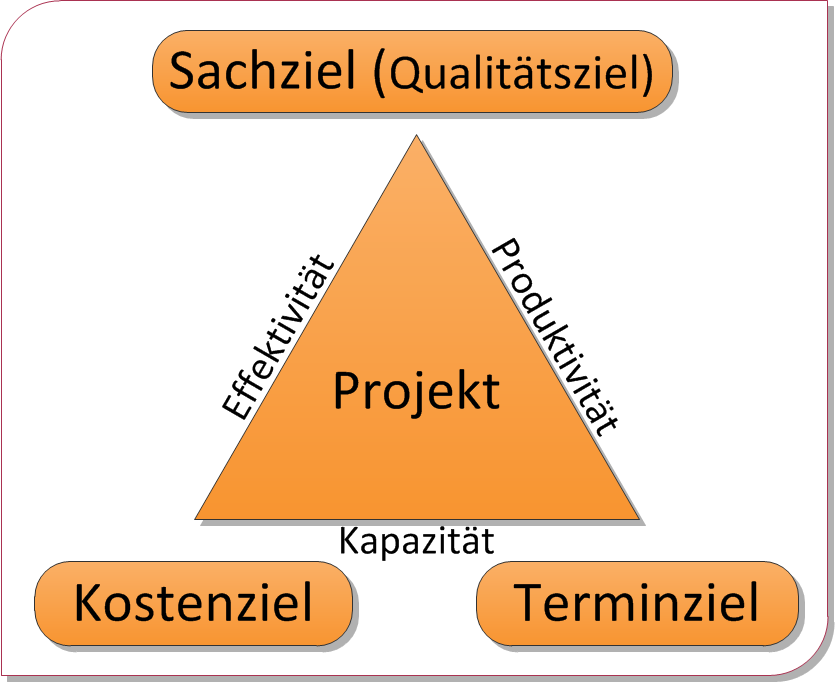
\includegraphics[width=0.4\textwidth]{Images/magischesDreieck.png}
\begin{center}
   {\footnotesize In Anlehnung an: \cite{Wischnewski1991}}
   \caption[Magisches Dreieck]{Magisches Dreieck}\label{abb2}
\end{center}
\end{floatingfigure}\noindent
Es stellt sich die Frage, welche Parameter entscheidend für den Erfolg eines Projektes sind. Aus den oben genannten Merkmalen lassen sich die Parameter Qualität des Ergebnisses (Sachziel), Kosten (Kostenziel) und Dauer (Terminziel) ableiten. Diese Ziele beeinflussen sich gegenseitig und bilden das so genannte „magische“ Dreieck der Projektorganisation (siehe Abbildung \ref{abb2} auf S. \pageref{abb2})\footnote{Vgl. \cite{Wegmann&Winklbauer2006}}
Typisch für viele Projekte ist, dass man anfangs nicht weiß, ob die angestrebten Ziele überhaupt erreicht werden können. Häufig wird der Zeitrahmen nicht eingehalten, die Kosten werden überschritten, oder man ist nicht in der Lage, die erhoffte Qualität zu erbringen\footnote{Vgl. \cite{Fiedler2008}, S.~3}.

Die Aufgabe des Projektmanagements besteht darin, dafür zu sorgen, dass das Vorhaben unter der Berücksichtigung der Projektziele durchgeführt wird. Das Projektmanagement nimmt dabei bestimmte Funktionen wie etwa Planung, Führung und Controlling wahr\footnote{Vgl. \cite{Bergmann&Garrecht2008}, S.~209}. Nach DIN 69901 versteht man unter dem Begriff  Projektmanagement: \label{69901Projektmgmt}\begin{quote}Projektmanagement ist die Gesamtheit von Führungsaufgaben, -organisation, -techniken und –mitteln für die Abwicklung eines Projekts.\end{quote}\par 

\subsection{Controlling}
\label{ssec:c}
Controlling hat sich in den letzten Jahren zu einer festen Institution in den Unternehmen entwickelt. Es gibt kaum ein Unternehmen, das keine eigene Abteilung oder zumindest Angestellte hat, die für das Controlling verantwortlich ist. Der Begriff Controlling ist allerdings sehr weit gefasst. Die Anforderungen in den Unternehmen sind so komplex, dass sich das Controlling dezentralisieren muss, um seine Aufgabe erfüllen zu können. Der Controller kann als ein \glqq Beifahrer\grqq  definiert werden, der den \glqq Fahrer\grqq (Manager) beim Steuern des \glqq Fahrzeugs\grqq \ (Unternehmen) unterstützt. Der Fahrer konzentriert sich auf das Steuern und auf die möglichen Reaktionen. Diese Aktivitäten verlangen seine volle Aufmerksamkeit und er kann keine anderen Tätigkeiten wie etwa Kartenlesen verrichten. Der Beifahrer ist freier als der Fahrer. Er kann daher nützliche Dinge tun, die den Fahrer unterstützen\footnote{Vgl. \cite{Pufahl2006}, S.~11}.\newpage
\begin{floatingfigure}[r]{0.37\textwidth} 
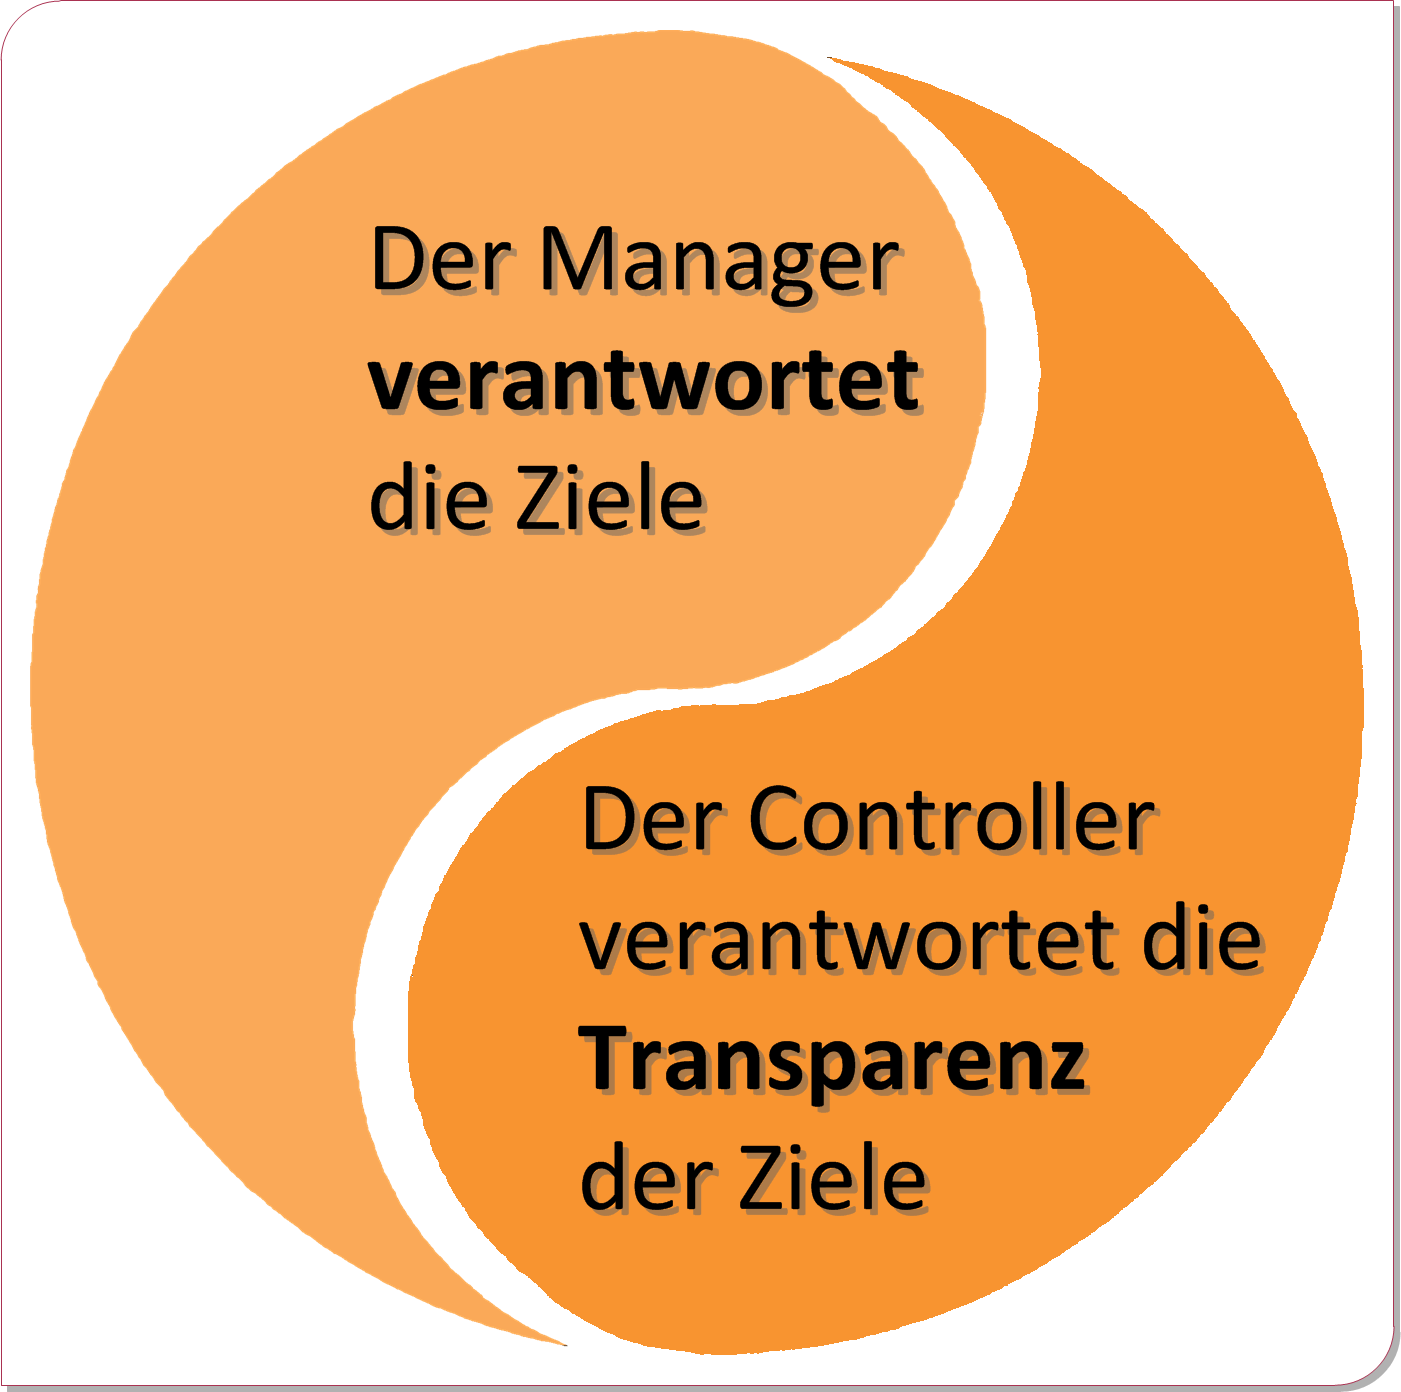
\includegraphics[width=0.37\textwidth]{Images/aufgabenabgrenzungLeiterController.png}
\begin{center}
   {\footnotesize In Anlehnung an: \cite{Fiedler2008}, S. 21}
   \caption[Management vs. Controlling]{Management vs. Controlling}\label{abb4}
\end{center}

%\end{figure}
\end{floatingfigure}\noindent
Controlling hat primär die Aufgabe, zwischen Planung, Kontrolle und Informationsversorgung zu koordinieren (so genannte systemkoppelnde Funktion des Controllings). Die Daten der Planung sind beispielsweise so aufzubereiten, dass eine Kontrolle möglich wird.  Auch innerhalb der Planung und Kontrolle sind Abstimmungen erforderlich. Es muss z. B. der Absatzplan mit dem Produktionsplan und dieser wiederum mit dem Investitionsplan koordiniert werden. Das Controlling stellt auch die Abbildung der strategischen Ziele in der operativen Perspektive sicher. Wichtig ist auch die Gestaltung der genannten Aufgabenbereiche, also die Schaffung von Strukturen und Prozessen. Die systembildende Funktion des Controllings regelt beispielsweise, welche Pläne zu erstellen sind und wie deren Kontrolle funktioniert. Hierzu werden die geeigneten Instrumente und Methoden, sowie die Verantwortlichen festgelegt\footnote{Vgl. \cite{Fiedler2008}, S.~10 f.}.
\subsection{Projektcontrolling}
\label{ssec:pc}
Die DIN 69901 beschreibt das Projektcontrolling als Regelkreis:\begin{quote}Sicherung des Erreichens der Projektziele durch: Soll-Ist-Vergleich, Feststellung der Abweichungen, Bewerten der Konsequenzen und Vorschlagen von Korrekturmaßnahmen, Mitwirkung bei der Maßnahmenplanung und Kontrolle der Durchführung.
\end{quote}
Für das Verständnis ist es wichtig, die Stellung des Projektcontrollings zum allgemeinen Unternehmenscontrolling und zum Projektmanagement herauszuarbeiten (Vgl. Abbildung \ref{abb3} auf Seite \pageref{abb3}). Die Begriffe Einzelprojektcontrolling, Multiprojektcontrolling und strategisches Projektcontrolling werden nicht einheitlich verwendet. Üblich ist es auch, das strategische Projektcontrolling als strategisches Multiprojektcontrolling oder Portfoliocontrolling zu bezeichnen.
\begin{figure}[htbp]
%\begin{floatingfigure}[r]{0.7\textwidth} 
\includegraphics[width=1\textwidth]{Images/stellungProjektcontrolling.png} 
\begin{center}
   {\footnotesize In Anlehnung an: \cite{Fiedler2008}, S. 13 u. 23}
   \caption[Stellung des Projektcontrollings]{Stellung des Projektcontrollings}\label{abb3}
\end{center}
\end{figure}
%\end{floatingfigure}
Die Abbildung \ref{abb3} auf Seite \pageref{abb3} zeigt, dass sich das Projektcontrolling als Bindeglied zwischen dem Unternehmenscontrolling und dem Projektmanagement wiederfindet.
Die Strategien, Ziele und Werte des Unternehmens werden so in die Gestaltung der Prozesse und Strukturen einfließen. Anders herum sind die Daten des Projektes für den Erfolg und die Liquidität des Unternehmens relevant. [...]tbd
Das Projektmanagement wird bei der Wahrnehmung der Führungsaufgaben und Koordination unterstützt\footnote{Vgl. \cite{Fiedler2008}, S.~13 f.}.

Zu unterscheiden sind Einzelprojektcontrolling, Multiprojektcontrolling und strategisches Projektcontrolling. Neben den unterschiedlichen strategischen bzw. operativen Ausrichtungen, sind diesen Bereichen auch unterschiedliche Aufgabenschwerpunkte zuzuordnen.
Ziel des Einzelprojektcontrollings ist es, das Projektmanagement so zu unterstützen, dass ein einzelnes Projekt bezüglich der Projektziele Qualität, Kosten und Zeit erfolgreich abgewickelt wird. Einzelprojektcontrolling orientiert sich an den Lebenszyklusphasen des Projektes und stellt dem Projektmanagement sowohl phasenspezifische wie auch phasenübergreifende Instrumente zur Verfügung.

Beim Multiprojektcontrolling werden mehrere Projekte mit unterschiedlichen Terminen und Fertigstellungsständen für eine Abrechnungsperiode zusammengefasst betrachtet. Ziel ist es, die Projektprogramm- und Projektablaufplanung unter Beachtung
\begin{compactitem}
\item der Kapazitätsgegebenheiten,
\item der Kosten- und Finanzwirkungen sowie
\item möglicher weiterer Nebenbedingungen(z. B. strategische Ziele des Unternehmens)
\end{compactitem}
zu einem gemäß den Bereichs- bzw. Unternehmenszielen bestmöglichen Gesamtgefüge zu koordinieren. Die Instrumente des Multiprojektcontrollings sind im Prinzip die gleichen wie beim Einzelprojektcontrolling, nur mit dem Unterschied, dass mehrere Projekte gleichzeitig bzw. zu einer Gruppe verdichtet betrachtet werden. Diese operativen Projektaspekte werden im Kapitel \ref{sec:opc} auf Seite \pageref{sec:opc} ausführlich behandelt.

Die Form des strategischen Projektcontrollings befasst sich mit strategischen Aufgabenstellungen des Projektmanagements. Dazu gehört die Bereitstellung von Informationen und Instrumenten zur effektiven Projektbewertung und Projektauswahl\footnote{Vgl. \cite{Fiedler2008}, S.~14--16}. Das strategische Projektkontrolling wird im nachfolgenden Kapitel \ref{sec:spc} detailliert beschrieben.



\abk{Balanced Scorecard}{ausgewogener Berichtsbogen zur Unterstützung der Operationalisierung und Implementierung der Strategie\footnote{Vgl. \cite{kaplan1997}, passim}}
\abk{Projekt-Scorecard}{auf die Belange der Projektarbeit angepasste Balanced Scorecard}

\section{Strategisches Projektcontrolling}
\label{sec:spc}
In diesem Kapitel werden die wesentlichen Aufgaben des Projektcontrollings im strategischen Projektmanagement erklärt. \\
Neben der strategischen Projektplanung und Vorgehensweise bei der Projektauswahl, wird ein besonderer Schwerpunkt auf die Managementmethode der Projekt-Scorecard zur Priorisierung und Steuerung von Projekten gelegt. Den Abschluss bilden Betrachtungen zur strategischen Kontrolle.
\subsection{Strategisches Projektmanagement}
Christian Kunz kommt zur Erkenntnis, dass in der Literatur die Bedeutung von Projekten zur Implementierung von Unternehmensstrategien weitgehend akzeptiert ist. Weiterhin bestünde Einigkeit, dass aufgrund der Vielzahl der Projekte zur Implementierung von Strategien sowie der inhaltlichen Verknüpfung dieser untereinander eine Führungsfunktion die Abstimmung und Kontrolle der Projektgesamtheit übernehmen sollte. Das strategische Projektmanagement entspricht somit einer Führungsfunktion und kann als strategisch bedeutend eingestuft werden\footnote{Vgl. \cite{Kunz2007}, S.~11}.
Für die Effektivität und Effizienz eines projektorientierten strategischen 
Management ist ein leistungsfähiges strategisches Projektcontrolling eine wesentliche Voraussetzung\footnote{Vgl. \cite{Foschiani1999}, S.~133}.
Weiterhin ist das strategische Projektmanagement vom Programm-Management sowohl inhaltlich als auch begrifflich abzugrenzen. Programm-Management orientiert sich an einer zeitlich befristeten Anordnung vieler Teilprojekte, die insgesamt ein Großprojekt darstellen und mit Ergebnisverantwortung verbunden sind. Nach Beendigung des Programms wird auch die temporäre Struktur des Programm-Managements abgebaut. Demgegenüber stellt das strategische Projektmanagement eine dauerhafte Steuerungseinrichtung im Unternehmen dar, die eng mit dem restlichen Führungssystem des Unternehmens verbunden ist. Wie in Abbildung ersichtlich wird, besteht ein Projektportfolio somit sowohl aus Einzelprojekten als auch aus Projekten, die Bestandteil eines Programms sind\footnote{Vgl. \cite{Kunz2007}, S.~21}.
\begin{figure}[htbp]
%\begin{floatingfigure}[htbpr]{0.43\textwidth} 
\begin{center}
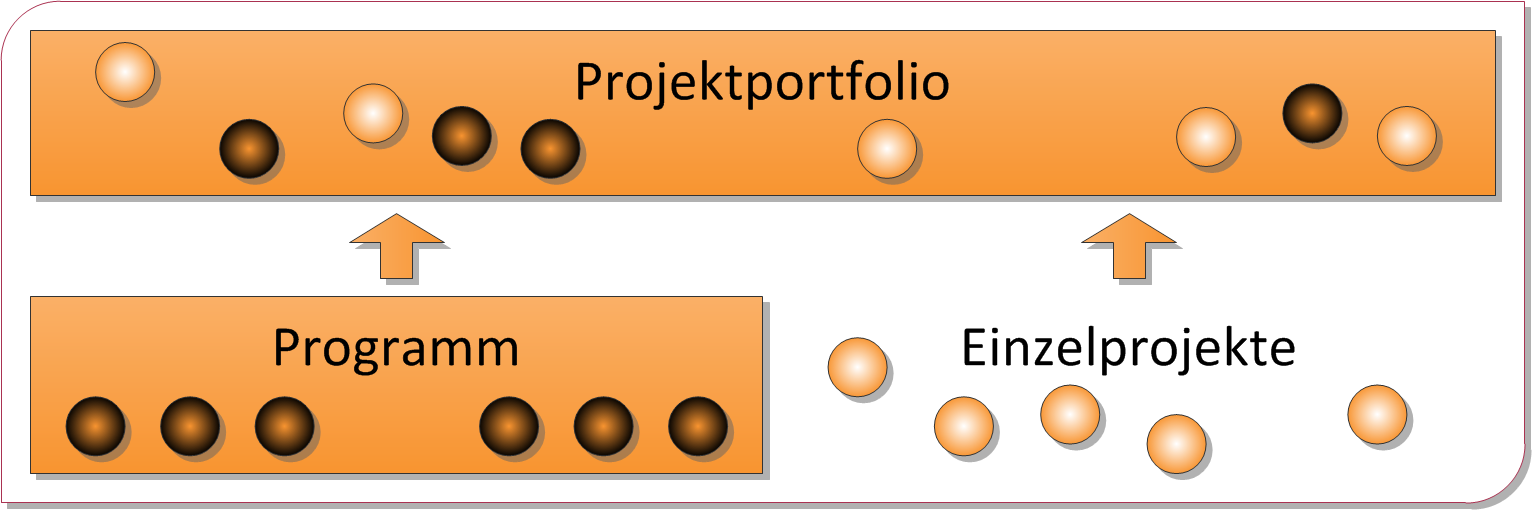
\includegraphics[width=0.8\textwidth]{Images/projektportfolio.png}
\label{abb5}

   {\footnotesize In Anlehnung an: \cite{Foschiani1999}, S.21--22]}
   \caption[Zusammenhang von Einzelprojekten, Programm und Projektportfolio]{Zusammenhang von Einzelprojekten, Programm und Projektportfolio}
\end{center}




\end{figure}
%\end{floatingfigure}

\subsection{Strategische Projektplanung}
\label{sec:SPP}
Grundlage der strategischen Projektplanung sind die Unternehmensziele, die wesentliche Auswahlkriterien für die Projekte liefern. Die Projekte müssen mit den strategischen Zielen harmonieren. Ein Unternehmen mit dem strategischen Ziel schnelles Wachstum durch Ausweitung des Marktanteils wird Projekte anders beurteilen als ein Unternehmen, das die Gewinnmaximierung durch Kostensenkung verfolgt.
Aufgrund der hohen Projektanzahl im Projektportfolio des strategisches Projektmanagements konkurrieren unterschiedliche Projekte um zumeist knappe Unternehmensressourcen\footnote{Vgl. \cite{Kunz2007}, S.~1}. Die Projektwünsche erreichen das Portfolio entweder Top-Down durch die Unternehmensleitung oder Bottom-Up durch die Fachbereiche. Dabei ist sicherzustellen, dass Projektideen nicht von vornherein abgeblockt oder bevorzugt werden. Jeder Vorschlag sollte zunächst die gleiche Chance haben. Ansonsten besteht die Gefahr, dass sinnvolle Vorhaben nicht realisiert werden\footnote{Vgl. \cite{Fiedler2008}, S~36}.
Zu Beginn der Projektportfolioplanung ist eine Gesamtbetrachtung aller Projekte anzustreben. Deswegen sollte man auch die bereits genehmigten und die laufenden Projekte in die Analyse einbeziehen. Es kann durchaus sein, dass schon genehmigte Vorhaben aufgrund der nachfolgenden Bewertung verschoben oder nicht realisiert werden\footnote{Vgl. \cite{Fiedler2008}, S.~39}.
\begin{figure}[htbp]
%\begin{floatingfigure}[htbpr]{0.43\textwidth} 
\begin{center}
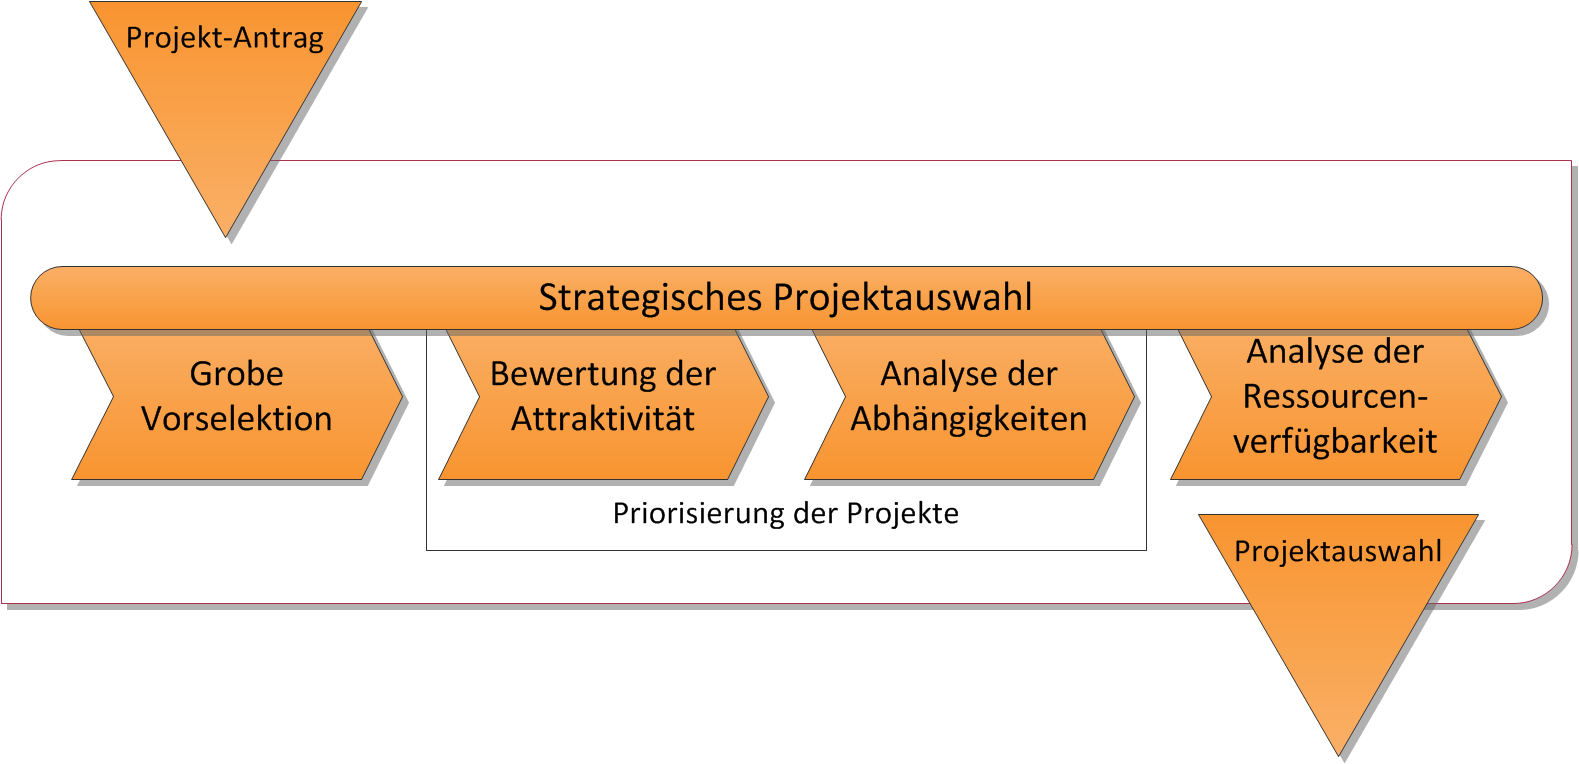
\includegraphics[width=0.8\textwidth]{Images/prozessProjektauswahl.png}
\label{abb6}

   {\footnotesize In Anlehnung an: \cite{Archer1999}, S. 208}
   \caption[Prozess der strategischen Projektauswahl]{Prozess der strategischen Projektauswahl}
\end{center}

\end{figure}
%\end{floatingfigure}
In der Abbildung \ref{abb6} auf Seite \pageref{abb6} wird der Prozess der strategischen Projektauswahl dargestellt. Die strategische Projektplanung nutzt diesen Ablauf, um die vorgeschlagenen Projekte im Einklang mit der Unternehmensstrategie auf die wirklich wichtigen zu beschränken. Die hierbei zum Einsatz kommenden Methoden liefern einheitliche Beurteilungskriterien und reduzieren die Gefahr, knappe Ressourcen zu verschwenden. Die strategische Projektplanung liefert so eine  Entscheidungsfundierung, auf Basis derer das Management die letztendliche Projektauswahl trifft\footnote{Vgl. \cite{Fiedler2008}, S.~85}.

Die grobe Vorselektion prüft neben der Machbarkeit, ob die Projektvorschläge den strategischen Zielen offensichtlich widersprechen. In dieser Phase kann es zur Definition von Muss-Projekten kommen. Dabei handelt es sich um Vorhaben, die z. B. aufgrund gesetzlicher Vorschriften unumgänglich sind\footnote{Vgl. \cite{Fiedler2008}, S.~41}.

Im Schritt Bewertung der Attraktivität wird die Attraktivität der Projekte für das unternehmen detailliert bewertet. Die wichtigsten Bewertungskriterien sind:
\begin{compactitem}
\item Strategische Bedeutung (Wettbewerbsvorteile, Kundenorientierung),
\item Dringlichkeit,
\item Wirtschaftlichkeit,
\item Risiko,
\item Kosten (Entwicklungskosten, Folgekosten),
\item Ressourcenbedarf\footnote{Vgl. \cite{Fiedler2008}, S.~41}.
\end{compactitem}
Rudolf Fiedler schreibt über die Aufgabe des Projektcontrollings bei der Bewertung der Attraktivität:
\begin{quote}
Das Projektcontrolling hat die Aufgabe, Hilfestellung beim Einsatz von Bewertungsinstrumenten zu geben und die Konsistenz der zur Beurteilung herangezogenen Daten zu prüfen.\footnote{\cite{Fiedler2008}, S. 42}
\end{quote}
Für eine Gesamtbetrachtung aller Einflussfaktoren der Projektbewertung bietet sich die Nutzwertanalyse an. Weitere Instrumente zur Bestimmung der Attraktivität sind auch Portfolios und Wirtschaftlichkeitsrechnungen. Ein weiterer wichtiger Bestandteil ist die Risikoanalyse, um das Erfolgspotenzial der Projekte abzuschätzen\footnote{Vgl. \cite{Fiedler2008}, S. 42}.
[s. Kommentar] %zu wenig? dann noch Bilder von Nutzwert, Risiko, Portfolios und Wirtschaftlichkeitsanalysen einfügen.

In der Analyse der Abhängigkeiten werden die gegenseitigen Einflüsse der Portfolioprojekte untersucht. Ein Projekt kann bereits in der Konzeptionsphase anderer Projekte zur veränderten Vorraussetzungen führen. Auch müssen manche Projekte mit anderen zusammen realisiert werden, da nur so das Gesamtziel erreicht werden kann. Gerade wenn verschiedene Projekte aufeinander aufbauen, hat dies ggf. signifikante Auswirkungen auf die Kosten der Umsetzungen.
Die Ergebnisse der Auswirkungen stehen also in einem kausalen Zusammenhang mit der Attraktivität und bestimmen gleichermaßen die Priorität der Vorhaben\footnote{Vgl. \cite{Fiedler2008}, S. 79}. 

Nachdem die Projekte vorselektiert, detailliert analysiert und priorisiert wurden, wartet die \glqq Hitliste\grqq der effektivsten Projekte aus die Zuteilung der meist knappen finanziellen Mittel und qualifizierten Ressourcen. Die Analyse der Ressourcenverfügbarkeit ordnet die erforderlichen Ressourcen nach Qualifikationsprofilen und die finanziellen Mittel nach den Budgets Projektklassen zu. Budgets für unterschiedliche Projektklassen werden gebildet, da gerade IT-Projekte oft große Teile des zur Verfügung stehenden Budgets aufzehren und so keine Mittel mehr für andere Projektarten zur verwendet werden können.
Ergebnis dieser Untersuchung kann auch sein, dass Projektstarts verschoben, Leistungsumfänge gekürzt oder gar laufende Projekte gestoppt werden\footnote{Vgl. \cite{Fiedler2008}, S.~81--82}.

\subsection{Strategische Projektkontrolle}
\begin{figure}[htbp]
%\begin{floatingfigure}[htbpr]{0.43\textwidth} 
\begin{center}
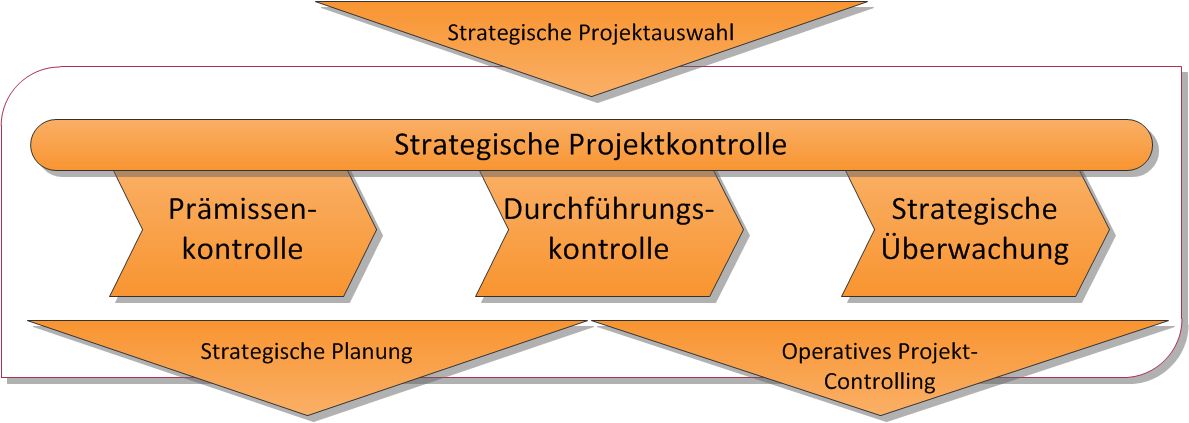
\includegraphics[width=0.8\textwidth]{Images/prozessStratKontrolle.png}
   %{\footnotesize In Anlehnung an: \cite{Steinmann&Schreyogg2000}, S. 221}
   \caption[Prozess der strategischen Projektkontrolle]{Prozess der strategischen Projektkontrolle}\label{abb6}
\end{center}

\end{figure}
%\end{floatingfigure}
Die strategische Projektkontrolle unterteilt sich in die drei wichtige Aufgaben\footnote{Vgl. \cite{Steinmann&Schreyogg2000}, S. 221}:
\begin{compactitem}
\item Prämissenkontrolle,
\item Durchführungskontrolle und
\item strategische Überwachung.
\end{compactitem}
Die Prämissenkontrolle untersucht während Projektauswahl und Projektdurchführung das gesamte Projektportfolio auf seine Ausgewogenheit und Stimmigkeit im Bezug auf die strategische Ausrichtung des Unternehmens. Sie stellt sicher, dass die in den Projektportfolios enthaltenen Projekte weiterhin den aktuellen strategischen Prämissen entsprechen. Hierzu sind gegebenenfalls einzelnen Projekte neu zu priorisieren\footnote{Vgl. \cite{Kunz2007}, S.~37}. 

Im Rahmen der Durchführungskontrolle werden Informationen von allen Portfolioprojekten generiert, um den Fortschritt der einzelnen Projekte zu verfolgen. Mittels Definition messbarer Meilensteine, deren Ist-Ergebnisse mit der ursprünglichen Zielsetzung verglichen werden, werden strategisch relevante Problemfälle innerhalb des Projektportfolios identifiziert. Bei signifikanten Abweichungen sind Gegenmaßnahmen einzuleiten\footnote{Vgl. \cite{Kunz2007}, S.~37}~\footnote{Vgl. \cite{Fiedler2008}, S.~87}. Geeigneter Methoden der Durchführungskontrolle sind z. B. Variationen der Balanced Scorecard (Projekt--Scorecard), Checklisten oder Portfiliotechniken (Mapping Grids).

Neben diesen Kontrollaktivitäten, die vor allem auf die Sicherstellung der zielgerichteten Durchführung von Projekten abzielen, fungiert die strategische Überwachung als ungerichtete flächendeckende Kontrolle als Ergänzung der beiden erstgenannten Kontrollen\footnote{Vgl. \cite{Fiedler2008}, S.~89}. Durch die Zusammenführung von Ergebniskontrolle und während der Projektdurchführung mitlaufender Wissensgenerierung werden die Projekte regelmäßig auf ihre Zielerreichung im Kontext der Unternehmensstrategien hin untersucht\footnote{Vgl. \cite{Kunz2007}, S.~37}.
%\subsection{Projekt-Scorecard}

\section{Operatives Projektcontrolling}
\label{sec:opc}
In diesem Kapitel wird das operative Projektcontrolling orientiert an den Lebenszyklusphasen eines einzelnen Projektes beschrieben. Die Sicht auf die Planung wird um die Aspekte der Steuerung und Kontrolle ergänzt.[...]tbd
\subsection{Operative Projektplanung}
\label{ssec:opp}
\begin{quote}
\glqq Projektplanung meint die systematische Informationsgewinnung über den zukünftigen Ablauf des Projektes und die gedankliche Vorwegnahme des notwendigen Handelns im Projekt.\grqq\footnote{\cite{Platz&Schmelzer1986}, S.~132}
\end{quote}
Die Projektplanung beschränkt sich nicht auf einen einmaligen Prozess am Anfang eines Vorhabens, sondern wird projektbegleitend durchgeführt\footnote{Vgl. \cite{Fiedler2008}, S.~100}. D. h. die Planung bezieht sich einerseits auf den Projektgegenstand und andererseits auf den Projektablauf\footnote{Vgl. \cite{Litke2007}, S.~153}. Im Verlauf der Projektrealisierung dient der Projektplan als Grundlage für Fortschrittskontrollen und Projektbewertungen, die ohne einen solchen Plan unmöglich wären. Der kontinuierlich den aktuellen Gegebenheiten angepasste Projektplan konvergiert zum Projektende gegen den Ist-Zustand\footnote{Vgl. \cite{Gubbels2006}, S.~8}
\begin{table}
\begin{center}
\caption[Überblick über die operative Projektplanung]{Überblick über die operative Projektplanung}

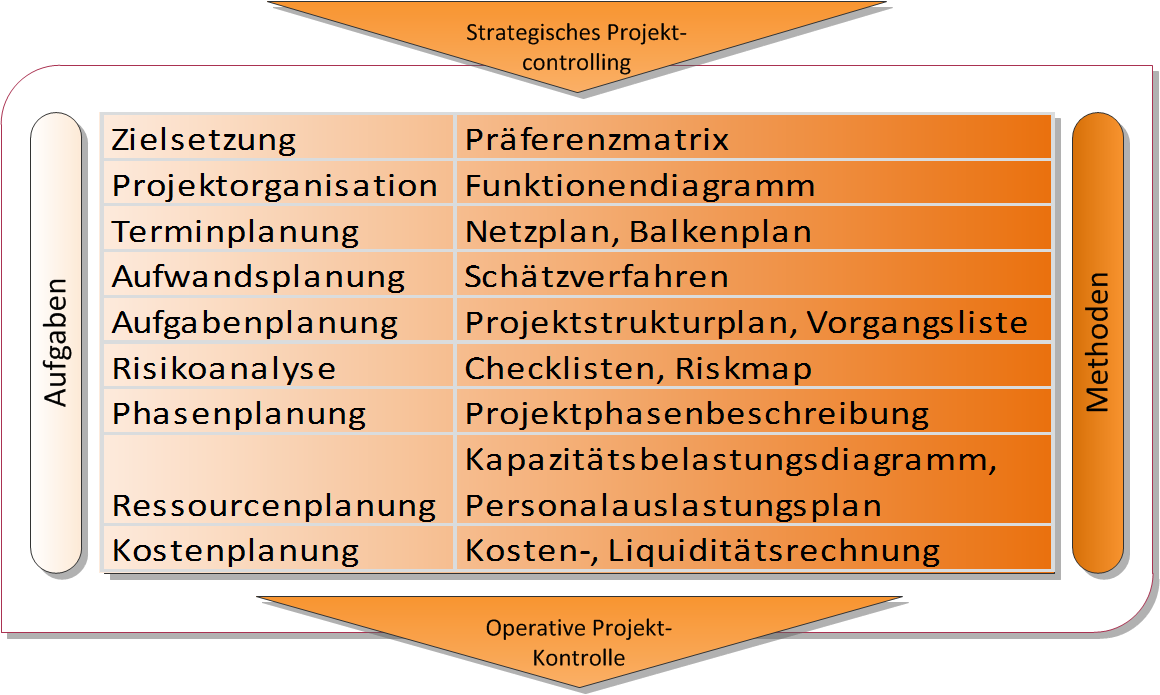
\includegraphics[width=0.8\textwidth]{Images/opPlanung.png}
\label{tbl1}

   {\footnotesize In Anlehnung an: \cite{Fiedler2008}, S. 100}
\end{center}

\end{table}

Die Tabelle \ref{tbl1} auf Seite \pageref{tbl1} zeigt einen Überblick über die verschiedenen Aufgaben und Methoden innerhalb der operativen Projektplanung. 
Der Projektleiter ist für die Planung verantwortlich\footnote{Vgl. \cite{Kuster&Huber2011}, S.~148}. Im Folgenden werden die Aufgaben des Projektcontrollings herausgestellt und abgegrenzt.

Die grundsätzlichen Regelungen für die Planungen wird durch das operative Projektcontrolling erarbeitet. Dazu gehört die verbindliche Vorgabe, dass kein Projekt ohne Projektauftrag mit Zielplanung gestartet wird.\footnote{Vgl. \cite{Fiedler2008}, S.~101}. 

%\begin{quote}
%Das Projektcontrolling kann Kriterien(z. B. Größe, Komplexität,Bedeutung des Projekts) für die Wahl der Projektorganisation erar-beiten.Im Rahmen der Planung wirdder Projektleiterunterstützt, um diefür das Projekt erforderlichen Personen zu finden. In der Matrixor-ganisation tritt manchmal das Problem auf,dass die Mitarbeiternicht in ausreichendem Maße von ihren Fachabteilungsaufgabenentlastet werden. Der Projektcontroller achtet deshalb frühzeitigdarauf,dass Vereinbarungen zwischen Projektleiterund Fachbe-reichsleitung zur Freistellung der Mitarbeiter getroffen und eindeu-tig dokumentiert werden.\footnote{\cite[S.~102]{Fiedler2008}}
%\end{quote}
%\begin{quote}
%Da die Aufgabenstruktur vieler Projekte vergleichbar ist, sollte dasProjektcontrollingeinen Standardprojektstrukturplan erarbeiten.Die Anpassung an einneues Projekt ist schnell durchführbar, indemeinfach die nicht benötigten Arbeitspaketeentferntund neue dazu-gefügt werden. So erhält man schnell einen aktuellen Planmit Aus-gangsdaten für die Termin- und Kostenplanung.Die folgende Abb. 83 zeigt im Überblick die Gliederung der Ebenendes Standardstrukturplans für das Projektgeschäft der FAG Kugelfi-scher AG  Co. KG. 
%Das Projektcontrolling kann auch formale Standards für die Defi-nition von Projektstrukturplänen vorgeben:• Eine Aktivität muss immer aus einem Hauptwort und einemVerbbestehen, z. B. "Bremsenprüfen".• Ein Meilenstein ist als Ereignis zu formulieren, z. B. "Bremsengeprüft".• Dieerste Ebene ist mit Großbuchstaben zuschreiben, um dieÜbersichtlichkeit zu erhöhen.• Auf der ersten Ebene dürfen keine Arbeitspaketeerscheinen.• Dieerste Ebene umfasst immer diegleichen, zentral vorgegebe-nen Standardvorgänge.• Essind höchstenssechs Gliederungsebenen zulässig. 
%Das Projektcontrolling hat im Rahmen der Koordination die korrek-te Definition der Meilensteine dahingehend zu prüfen, ob sie mitdem Projektauftrag korrespondierenoder vertraglich zugesicherteLeistungstermine berücksichtigen. Außerdemmuss die Vollstän-digkeit des Projektstrukturplans begutachtet werden. Technischorientierte Projektleiter übersehen schnell vertriebliche und organi-satorische Aufgaben.Der Projektcontrollerunterstützt darüber hinaus die Abstimmungder Rahmen- und Detailpläne.\footnote{\cite{Fiedler2008}}
%\end{quote}\begin{quote}
%Als gestaltende Maßnahme muss das Projektcontrollingeine Ter-minplanung mit ausreichendem Detaillierungsgrad für jedesProjekt verbindlich fordern. Ergänzend sollten Empfehlungen fürden Einsatzvon Balkenplänen und Netzplandiagrammen formuliertwerden. Hinweise auf geeignete DV-Instrumente gewährleistenine effiziente und einheitliche Terminplanung.Der Projektcontroller kann auch die Machbarkeit des Terminplansprüfen. Insbesondere sollteer darauf achten, ob genügend Ressour-en zu den geplanten Zeitpunkten bereitstehen. Es ist auch sicher zutellen,dass die Ressourcenprojektübergreifend entsprechendderProjektprioritätenoptimal eingesetzt werden.Ein besonderes Augenmerk sollte der Projektcontroller auf dieein-geplanten Pufferrichten.\footnote{\cite[S.~130]{Fiedler2008}}
%\end{quote}\begin{quote}
%Das Projektcontrolling sollte die realistische Ermittlung und zen-trale Dokumentation der freien Kapazitäten sicherstellen. Damitwird auch eine ungleichmäßige Ressourcenauslastung vermieden. Inder Praxis kommt es immer wieder vor,dass einige Mitarbeiter zumehr als 100 Prozent ausgelastetsind, während andere noch freieKapazitäten haben.Diefür ein Projekt zur Verfügung stehende Zeit eines Mitarbeiterswird manchmal zu optimistisch gesehen. Gründe sind:• Es wirddiegesamte Bruttoarbeitszeit eingeplant.• Offiziell abgeschlossene Projekte binden weiterhin Kapazitätendes Mitarbeiters.• Urlaub und Krankheitstage werden übersehen. 
%Das Projektcontrolling sollte dazu beitragen,diese Probleme auf-zudecken.Erkennt der Projektcontroller Engpässe, muss er dafürsorgen,dassdiesefrühzeitig kommuniziert undbeseitigt werden.Es ist vor allem beiknappen Ressourcen erforderlich,dass eine pro-jektübergreifende Koordination des Mitarbeitereinsatzes erfolgt.Wertvoll ist es in dieser Situation, wenn die Prioritäten der Projektebekanntsind (vgl. Abschnitt 2.1).Der Projektcontrollersollte auch dafür Sorge tragen,dass dieein-zelnen Mitarbeiter nicht in zu vielen Projekten eingesetzt werden.Verplant man den Mitarbeiter inmehr als fünf Projekten, sindderKoordinierungsaufwand unddie durch den Wechsel zwischen denverschiedenen Aufgaben bedingten "geistigen Rüstzeiten" zu hoch.Wenn ein Mitarbeiter mit weniger als20 Prozent zur Verfügungsteht, ist auch das Interessefür das Projekt gering.In einer Projektmatrixorganisation,bei der ein Mitarbeiter nebendem Projekt auch noch sein Tagesgeschäft erledigenmuss, ist vonvornherein sicherzustellen,dass er in seiner Fachabteilung auchimerforderlichen Umfangentlastet wird. Geschieht das nicht, wirdderMitarbeiterschnell überfordert, mit der Folge,dass seine Motivationim Projektsinkt. Um diese Situation zu vermeiden, kann der Pro-jektcontroller einen Kontrakt zwischen ProjektleiterunddenAbteilungsleitern anregen, in dem diese sich verpflichten,die Mit-arbeiter entsprechend ihrer Projekteinplanung vom Tagesgeschäftfreizustellen.\footnote{\cite[S.~152--153]{Fiedler2008}}
%\end{quote}


\subsection{Operative Projektkontrolle}
Projektkontrolle hat die Aufgabe der Schaffung von Transparenz mittels eines effizienten Reportings und die Entscheidungsvor-- und --nachbereitung.\\Voraussetzung sind eine realistische, vollständige und nachvollziehbare Projektplanung (Vgl. Kapitel \ref{ssec:opp}). Den quantifizierbaren Größen der Projektkontrolle sind die Bewertungsdimensionen des magischen Dreieck (Vgl. Abb. \ref{abb2}, S. \pageref{abb2}) zu Grunde gelegt\footnote{Vgl. \cite{Bergmann&Garrecht2008}, S.~228}. Um mögliche Abweichungen vom geplanten Projektablauf zu erkennen, werden die Ist-Werte den ursprünglich geplanten Werten gegenübergestellt. Kommt es zu Abweichungen vom Plan, so erfolgt eine erneute Projektplanung auf Grundlage der aktualisierten Daten. Besteht die Gefahr, dass wichtige Abschlusstermine nicht eingehalten oder dass bestimmte Kostenziele überschritten werden, muss das Projektmanagement Maßnahmen entwickeln, um auf solche Abweichungen geeignet reagieren zu können\footnote{Vgl. \cite{Zimmermann&Rieck&Stark2006}, S.~107}
\begin{table}
\begin{center}
\caption[Elemente der Projektkontrolle]{Elemente der Projektkontrolle}

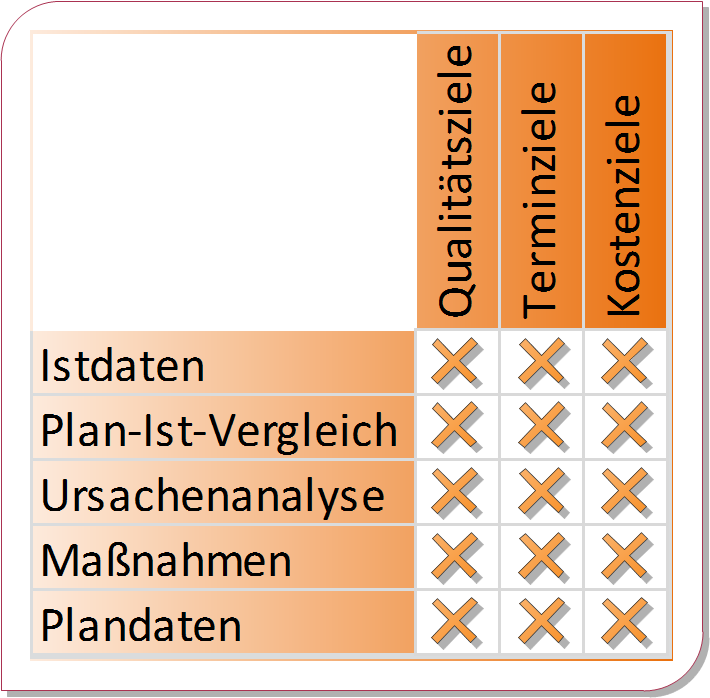
\includegraphics[width=0.4\textwidth]{Images/elementeSteuerung.png}
\label{tbl2}

   {\footnotesize In Anlehnung an: \cite{Fiedler2008}, S. 177}
\end{center}

\end{table}
Die Abbildung \ref{abb8} auf Seite \pageref{abb8} zeigt das Zusammenspiel der operativen Projektplanung und -kontrolle als Fundierung der Projektsteuerung. 
Die Projektkontrolle beinhaltet folgende Aufgaben(vgl. Abb. \ref{abb8})\footnote{Vgl. \cite{Fiedler2008}, S. 176}:
\begin{compactitem}
\item Ermittlung der Istdaten,
\item Gegenüberstellung der entsprechenden Plandaten,
\item Untersuchung der aufgetretenen Abweichungenmit dem Ziel, deren Ursachen herauszufinden, und gegebenenfalls
\item Planung und Einleitung von Gegenmaßnahmen.
\end{compactitem}
\begin{figure}[htbp]
%\begin{floatingfigure}[r]{0.7\textwidth}
\begin{center}
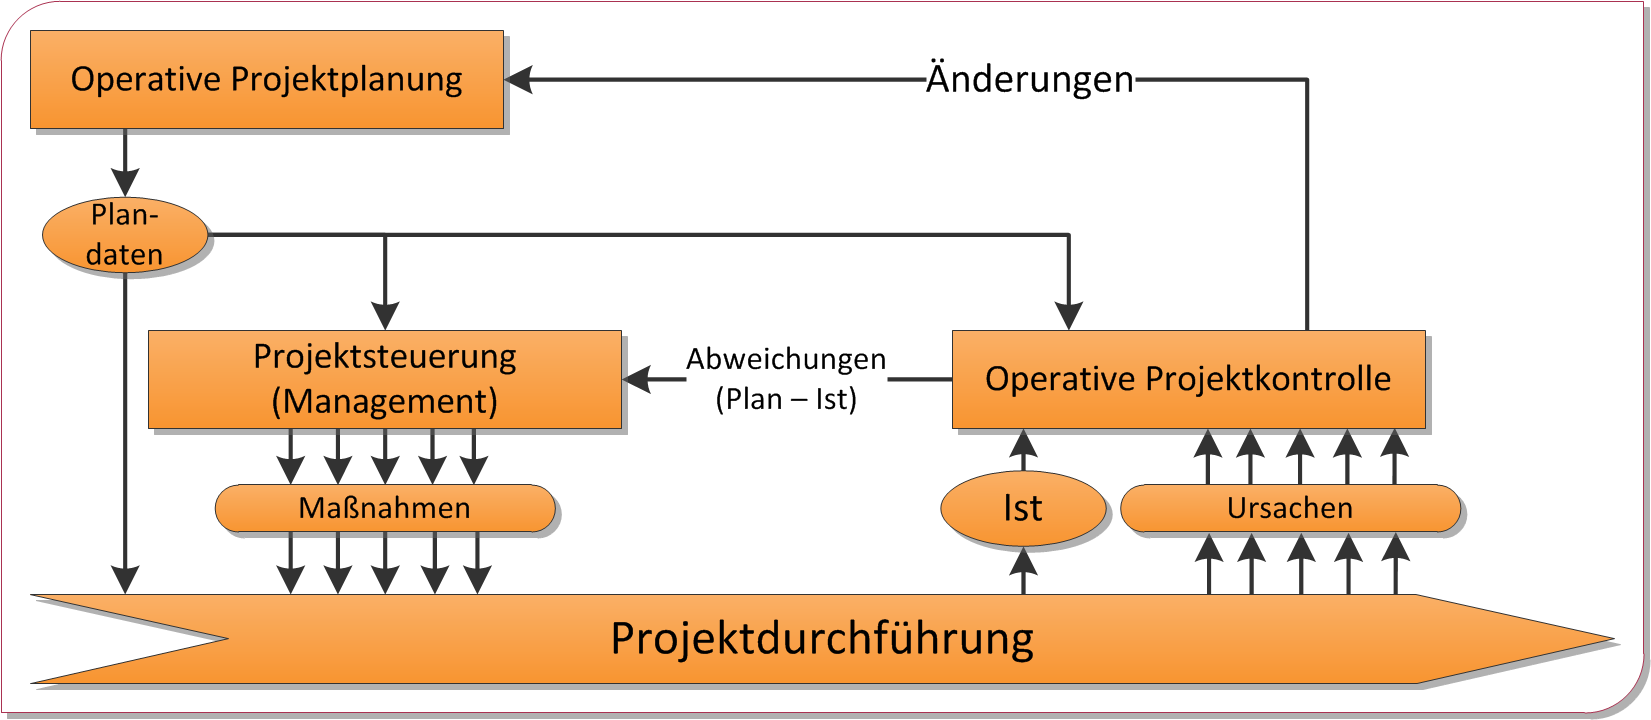
\includegraphics[width=1\textwidth]{Images/Steuerung.png}
{\footnotesize In Anlehnung an: \cite{Litke2007}, S. 84}
\caption[Modell der Projektlenkung]{Modell der Projektlenkung}\label{abb8}
\end{center}
\end{figure}
%\end{floatingfigure}
Nach Frank Lüschow und Elke Zitzke ist der Projektleiter auf die realistische Einschätzung seiner Teammitglieder angewiesen, um den Ist-Zustand im Projekt realistisch einschätzen zu können. An dieser Stelle ist der Projektleiter auf seine eigene und die Intuition seiner Teammitglieder angewiesen. Um an diese Informationen heranzukommen, muss er laufend aktiv Kontakt zu seinen Teammitgliedern halten. Diese Methode wird von den Autoren zusammengefasst als:\begin{quote}\glqq Controlling by walking around\grqq\footnote{\cite{Luschow&Zitzke2004}, S.~102}\end{quote}
Diese Methode ist nach Lüschow und Zitzke ein Teil der Kontrolle und wird durch messbare Daten gestützt\footnote{Vgl. \cite{Luschow&Zitzke2004}, S.~101--102}. Rudolf Fiedler bewertet die intuitive Einschätzung des Projektleiters und der Mitarbeiter weitaus kritischer. Er nimmt Bezug auf das 90\%- oder Fast-schon-fertig Syndrom und gibt zu Bedenken, dass der erreichte Fertigstellungsgrad oft zu hoch eingeschätzt wird, obwohl eine nicht mehr auszugleichende Planabweichung vorliegt\footnote{Vgl. \cite{Litke2007}, S.~181--182)}. \abk{90\%-Syndrom}{häufige Fehleinschätzung des Fertigstellungsgrades}
Unumstritten ist, dass für effizientes Projektcontrolling nicht nur ex-post 
durch Kontrolle und Überwachung Abweichungen festzustellen, sondern das 
Auftreten von Abweichungen antizipativ erst gar nicht entstehen zu lassen. Für diesen proaktiven Ansatz der Projektsteuerung empfiehlt es sich die Trends des Fortschritts in Besprechungen mit dem Projektteam regelmäßig abzufragen\footnote{Vgl. \cite{Bergmann&Garrecht2008}, S.~229}. 
\subsubsection{Einhaltung des Terminziels}
Eine Form der Darstellung des Plan-Ist-Vergleichs der Terminerreichung ist die Meilenstein-Trendanalyse (Abbildung \ref{abb9}, Seite \pageref{abb9}). In dieser Form der Darstellung wird die Erreichung der Meilensteine aufgeführt. An den Achsen werden die im Projektplan festgelegten Meilensteine (Ordinate) und die Berichtstermine (Abszisse) in zeitlich aufsteigender Folge eingetragen. Bei Erreichen der jeweiligen Berichtstermine wird die Abbildung weiter vervollständigt. Wenn im Laufe des Projektes die Planeinhaltung nicht mehr realistisch erscheint und es eine aktualisierte Erwartung gibt, so wird auf den neuen Erkenntnissen ein aktualisierter Plan aufgesetzt. Dieser Ausblick wird Forecast \abk{Forecast}{Ausblick/Prognose auf erwartete Ergebnisse nach aktuellen Erkenntnissen} genannt, in den Spalten zu den jeweiligen Berichtsterminen eingetragen und mit einer Linie verbunden\footnote{Vgl. \cite{Wegmann&Winklbauer2006}, S.~191--192}. Auf Basis des Kurvenverlaufs ist eine Termineinschätzung möglich\footnote{Vgl. \cite{Litke2007}, S.~156}:
\begin{compactitem}
\item Fallender Verlauf: Termin wird unterschritten.
\item Waagerechter Verlauf: Termin wird eingehalten.
\item Ansteigender Verlauf: Termin wird überschritten.
\end{compactitem}

\begin{figure}[htbp]
%\begin{floatingfigure}[r]{0.7\textwidth}
\begin{center}
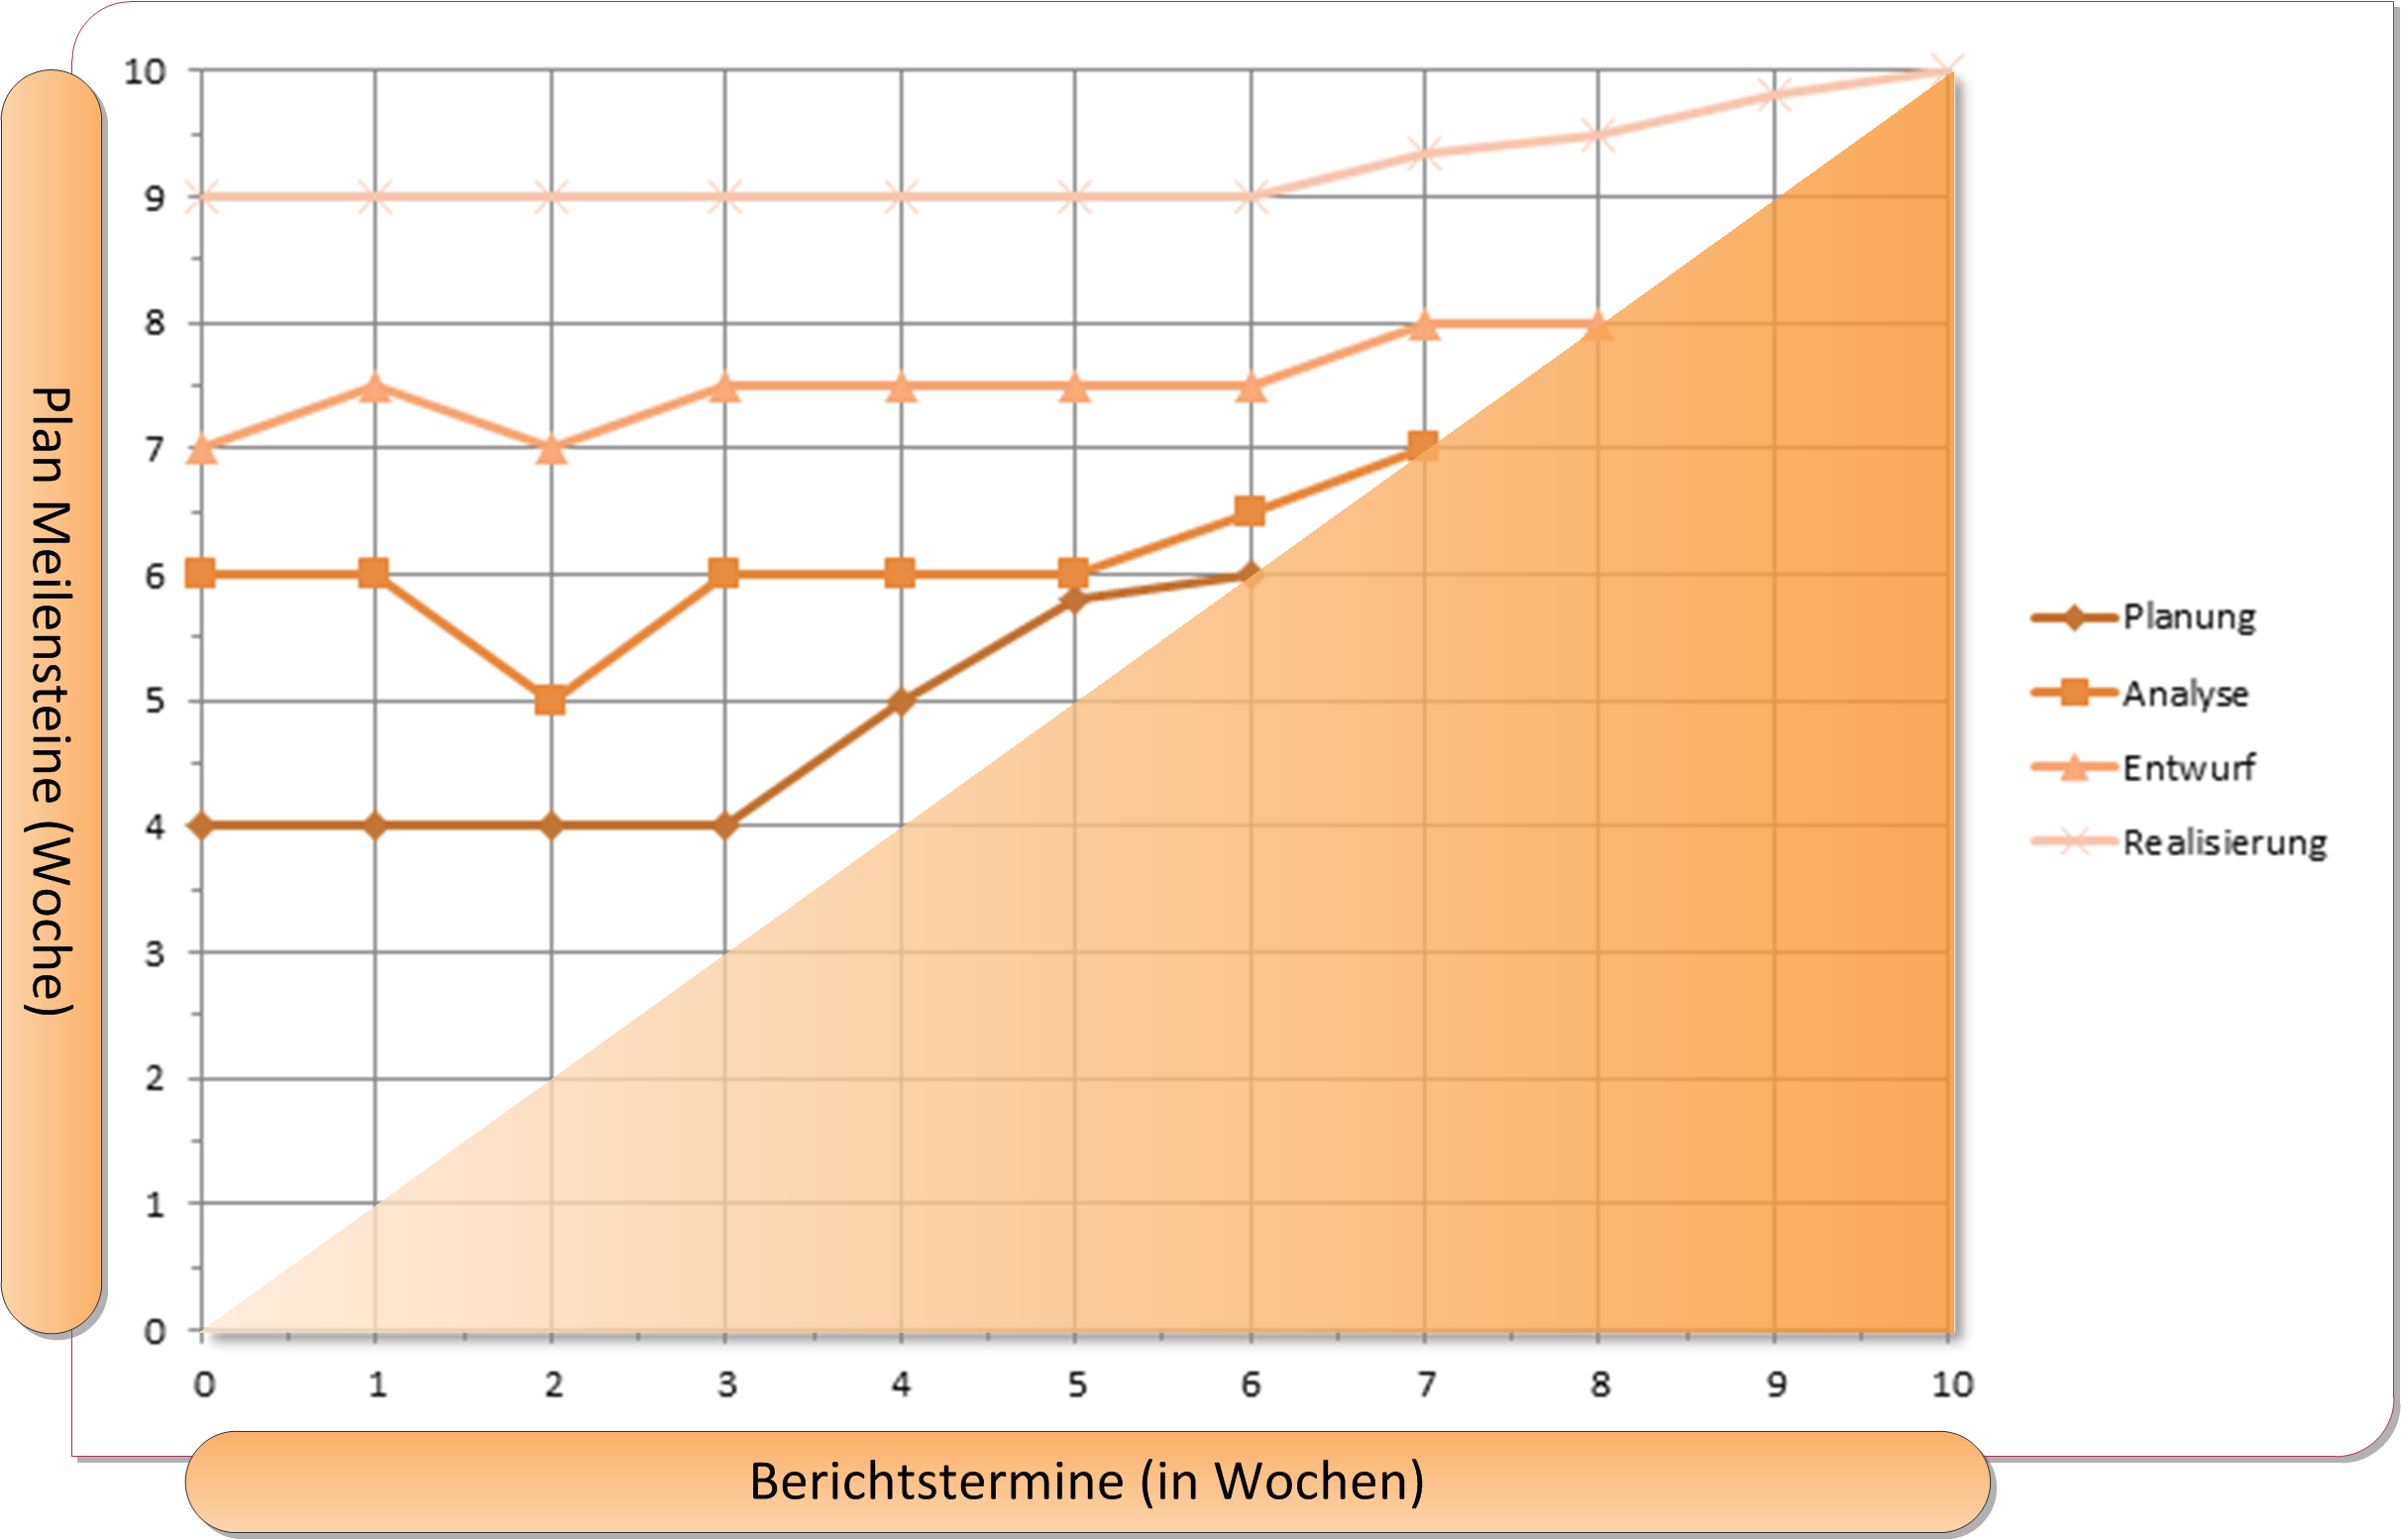
\includegraphics[width=0.8\textwidth]{Images/trendAnalyse.png}\\{\footnotesize In Anlehnung an: \cite{Blazek2001}, S. 152}
\caption[Meilenstein-Trendanalyse]{Meilenstein-Trendanalyse}\label{abb9}
\end{center}
\end{figure}
%\end{floatingfigure}

\subsubsection{Einhaltung des Qualitätsziels}
Für die Erfassung des Qualitätsziels stehen eine Reihe von Methoden und Techniken zur Verfügung. Eine besonders einfache Methode ist die Meilensteinmethode. Man zählt die bisher erreichten Meilensteine und setzt sie mit der Gesamtzahl der Meilensteine in Bezug. Sie die Meilensteine genügend differenziert, kann diese Form der Erfassung zufrieden stellende Ergebnisse liefern. Die Planabweichung wird dabei durch die zeitliche Bindung der Meilensteine deutlich und kann durch die Division der Ist- durch die Planwerte als Kennzahl des Fortschrittsgrades dargestellt werden\footnote{Vgl. \cite{Fiedler2008}, S.~182}.

Genauere Ergebnisse können mit dem Fokus auf die geplanten Arbeitspakete erzielt werden. Es wird die Planmäßigkeit der abgeschlossenen Arbeitspakete bewertet (0/100-Methode). Alternativ kann auch der Fortschritt innerhalb eines Arbeitspaketes bewertet werden. Man wählt hier Vorgehensweisen wie die 0/50/100-Methode, um dem 90\%-Syndrom angemessen zu begegnen\footnote{Vgl. \cite{Fiedler2008}, S.~183}.
Ein Beispiel zur Darstellung des aktuellen Projektfortschritts in MS-Project ist im Anhang 2 (Kapitel \ref{sec:Anhang2}, Seite \pageref{sec:Anhang2}) zu finden.

Oft wird die bereits erbrachte Leistung zu positiv eingeschätzt. Es bietet sich an, die noch zu erbringende Leistung als zukunftsorientierter Indikator der Qualität zu wählen\footnote{Vgl. \cite{Luschow&Zitzke2004}, S.~102}. Die Effort-Expended-Methode gibt den Leistungsmäßigen Fortschrittsgrad (FG) nach folgender Formel aus\footnote{Vgl. \cite{Fiedler2008}, S.~183}: $FG = \frac{Istaufwand*100}{Vorraussichtlicher Gesamtaufwand}$

\subsubsection{Einhaltung des Kostenziels}
Die Kostenkontrolle legt den Fokus auf die zum aktuellen Zeitpunkt erwarteten Kosten und vergleicht sie mit den tatsächlich angefallenen Kosten. Die Voraussetzung für aussagekräftige Auswertungen sind eine hohen Planungs- und Erfassungsqualität der Kosten. Eine einfache Variante eines Plan-Ist-Vergleich ist im Anhang 1 (Kapitel \ref{sec:Anhang1}, Seite \pageref{sec:Anhang1}) zu finden. Die Abbildung \ref{abb10} auf der Seite \pageref{abb10} zeigt eine zusammengefasste Sicht mit Forecast aus der Perspektive des gesamten Projektes\footnote{Vgl. \cite{Wegmann&Winklbauer2006}, S.~182--183}.
\begin{figure}[htbp]
%\begin{floatingfigure}[r]{0.7\textwidth}
\begin{center}
\includegraphics[width=0.8\textwidth]{Images/Forecast.png}\\{\footnotesize In Anlehnung an: \cite{Blazek2001}, S. 142}
\caption[Kostentrendanalyse]{Kostentrendanalyse}\label{abb10}
\end{center}
\end{figure}
%\end{floatingfigure}


\subsubsection{Earned Value Analyse}
\begin{table}[htbp]
%\begin{floatingfigure}[r]{0.7\textwidth}
\begin{center}
\caption[Abkürzungen Earned Value Analyse]{Abkürzungen Earned Value Analyse}\label{tbl3}
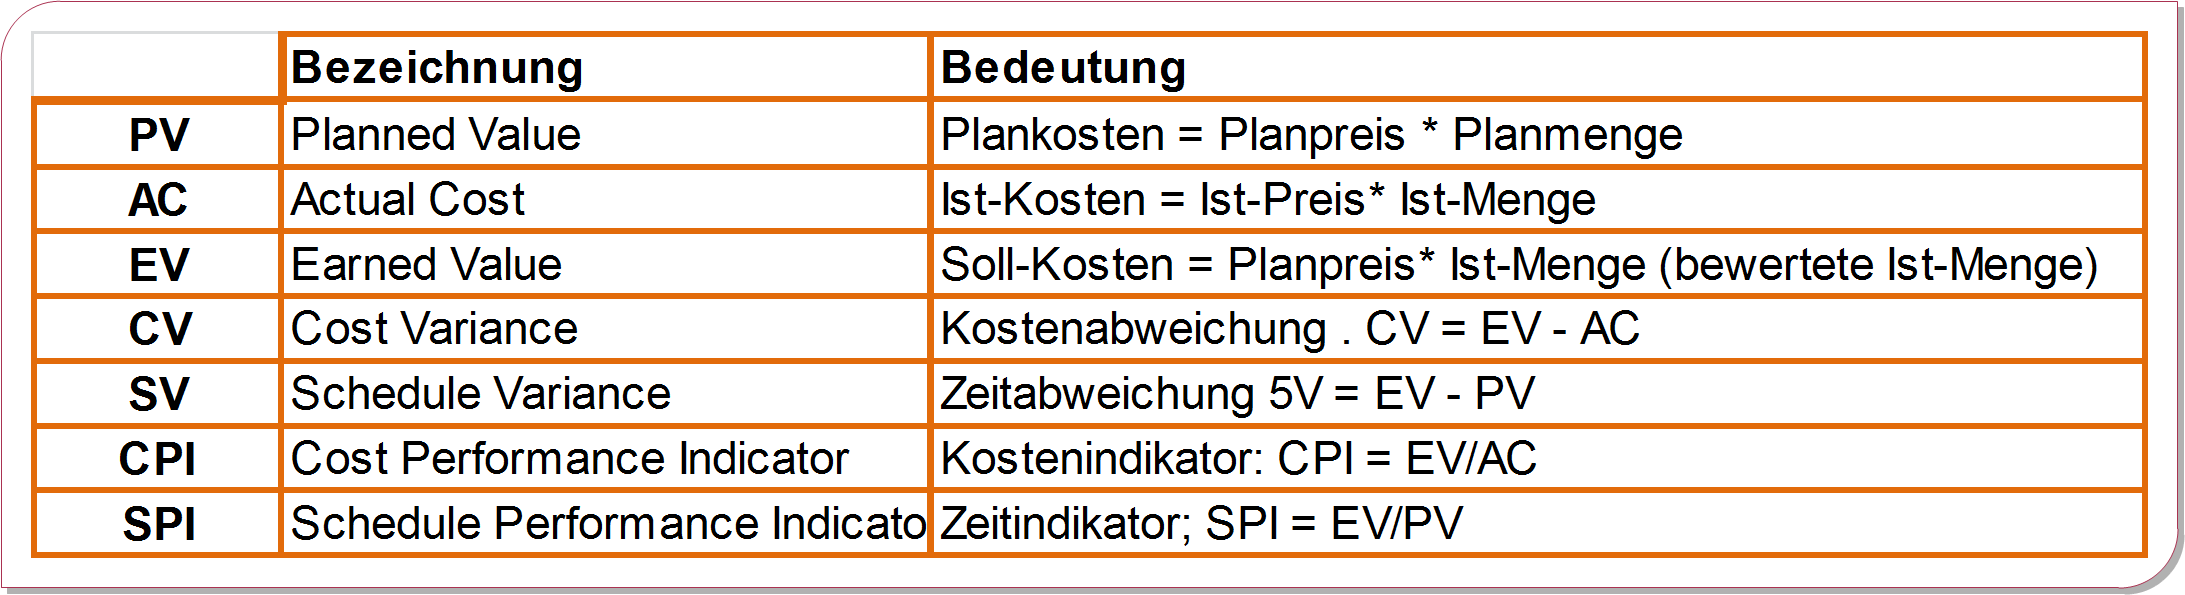
\includegraphics[width=0.8\textwidth]{Images/ev.png}\\{\footnotesize In Anlehnung an: \cite{Drews&Hillebrand2007}, S.~233}
\end{center}
\end{table}
In den vorangegangenen Kapiteln wurden Methoden aufgezeigt, die die Dimensionen des magischen Dreiecks einzeln überwachen. Am Beispiel der Kostenanalyse in Abbildung \ref{abb9} auf Seite \pageref{abb9} kann man nicht erkennen, ob die höheren Kosten zum Zeitpunkt der Erfassung auf einen schnellere oder eine unwirtschaftliche Leistungserbringung (Qualitätsziel) zurückzuführen ist. 
Das Beispiel verdeutlicht, dass die Kostenkontrolle auch die Erfüllung des Qualitätsziel mit einbeziehen muss. Dies erreicht man durch den Ausweis von Sollkosten für jedes Arbeitspaket. Das sind diejenigen Kosten, die für eine gegebene Leistung zum planmäßigen Termin anfallen dürfen. Man spricht auch vom so genannten Earned Value\footnote{Vgl. \cite{Fiedler2008}, S.~198}.
Die Earned-Value-Analyse berücksichtigt alle drei Dimensionen des magischen Dreiecks. Sie bedient sich dazu folgenden Kategorien: den Ist-Kosten, den Plankosten und den Soll-Kosten (Earned Value). Mit diesen drei Kategorien ermittelt die Earned-Value-Analyse die Kostenabweichung (Cost Variance) im Projekt. Die Kennzahl der Zeitabweichung wird als Schedule Variance bezeichnet. Die Kostenabweichung errechnet sich aus der Differenz der Soll-Kosten zu Ist-Kosten und zeigt die Abweichung der tatsächlichen Kosten zu den geplanten Kosten der erreichten Qualität. Die Zeitabweichung ermittelt sich aus der Differenz von Soll-Kosten - Plankosten\footnote{Vgl. \cite{Drews&Hillebrand2007}, S.~232}.
%\end{floatingfigure}
\begin{figure}[htbp]
%\begin{floatingfigure}[r]{0.7\textwidth}
\begin{center}
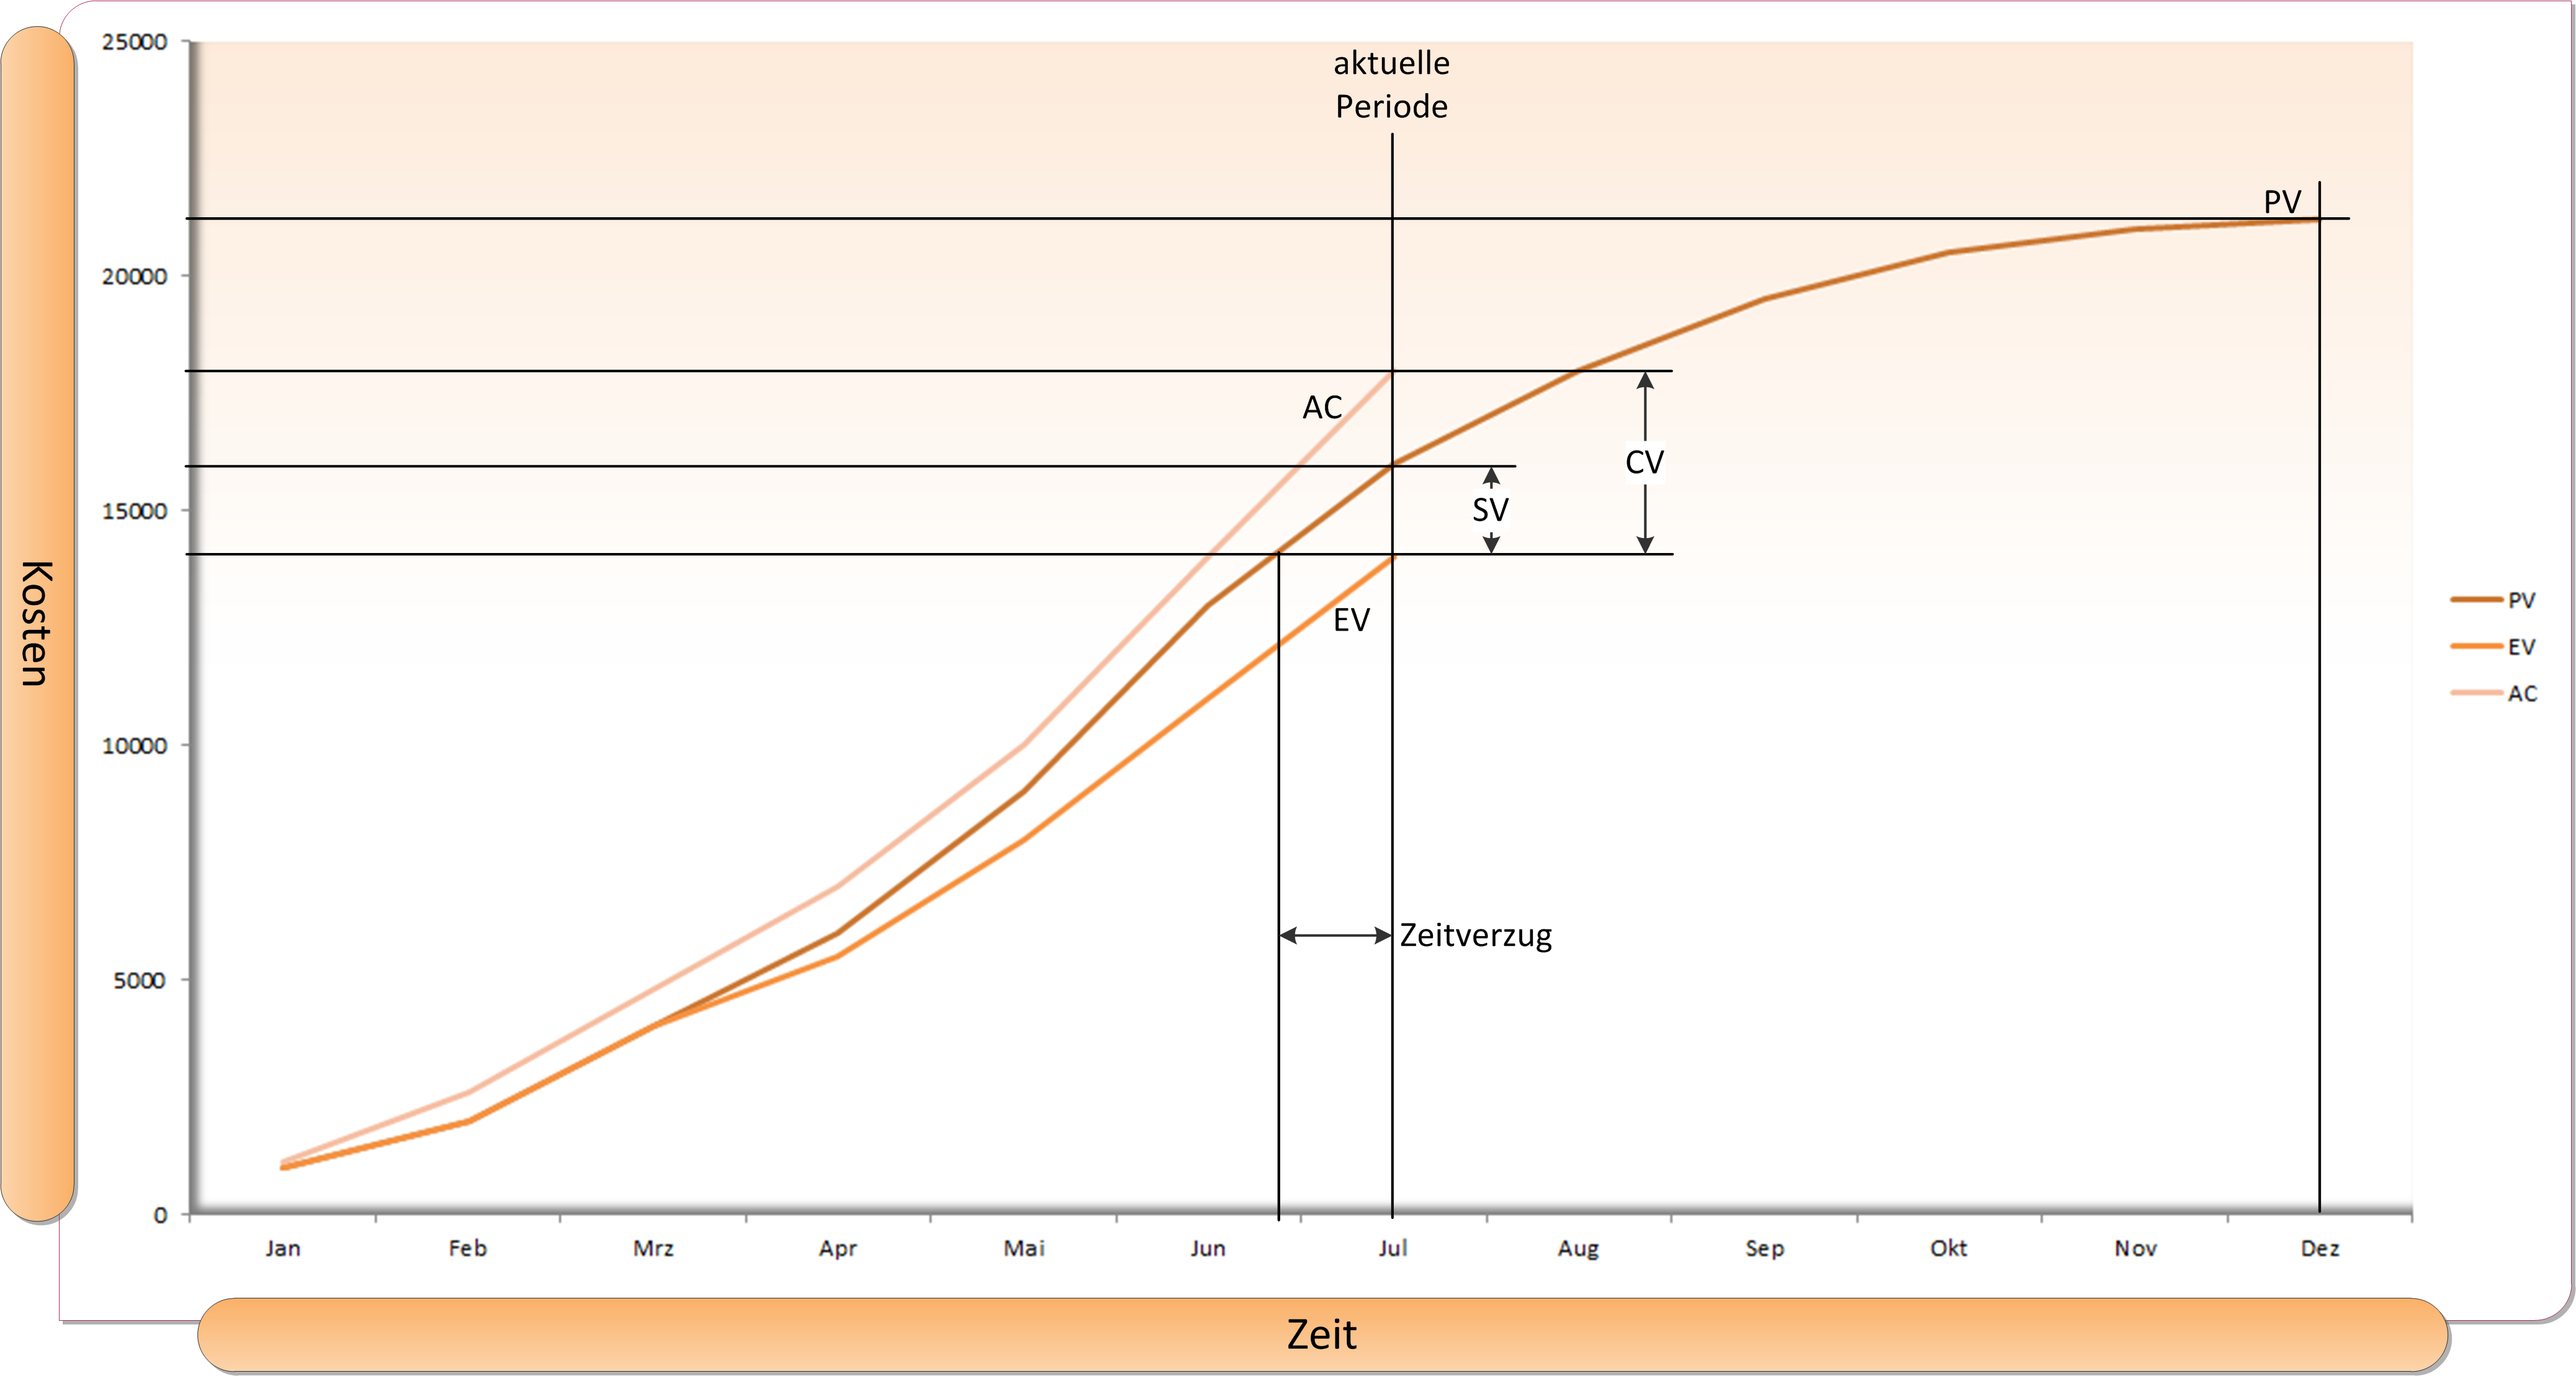
\includegraphics[width=1\textwidth]{Images/eva.png}\\{\footnotesize In Anlehnung an: \cite{Drews&Hillebrand2007}, S. 234}
\caption[Earned Value Analyse]{Earned Value Analyse}\label{abb11}
\end{center}
\end{figure}
%\end{floatingfigure}

Die Abbildung \ref{abb11} auf Seite \pageref{abb11} zeigt die Anwendung des Kennzahlensystems aus Tabelle \ref{tbl3} auf Seite \pageref{tbl3}. Mit den Größen der Earned Value Analyse lassen sich wie in der Meilensteintrendanalyse Aussagen zur Terminerreichung und wie in der Kostentrendanalyse Aussagen zum Kostenverlauf machen. Alle drei Werkzeuge bilden gemeinsam ein wichtiges Instrumentarium, um absolute Zahlen und Trends ermitteln zu können\footnote{Vgl. \cite{Gubbels2006}, S.~34}. 
\section{Fazit}
ERP-Software für das Finanzmanagement optimiert Abläufe des betrieblichen Rechnungswesen. Die SAP ERP-Anwendungen FI und CO können mit allen anderen Komponenten der Wertschöpfungskette integriert werden. Sie sparen Kosten und Zeit durch die Automatisierung von Geschäftsprozessen und schaffen im Rechnungswesen mehr Vertrauen durch eine zuverlässige Kontrolle finanzieller Risiken. 

Die SAP ERP Financials Module FI und CO sind elementare Bestandteile der Betriebswirtschaft und in jedem Unternehmen einsetzbar. Andere  Standard- oder eigenerstellte Softwarelösungen haben in deutschen Großunternehmen fast keine Bedeutung mehr\footnote{Vgl. \cite{Gleich2010}, S. 58}. Sie erfüllen sowohl die Vorgaben der gesetzlich vorgeschriebenen externen Rechnungslegung, als auch die vielfältigen Anforderungen an interne Analysen und Reportings im internen Rechnungswesen. 

Das Konzernprogramm One.ERP der Deutschen Telekom AG setzt ein Prozess-Tool um, das flexibel, schnell, standardisiert und kosteneffizient ist. Dies hat den wesentlichen Vorteil, dass unabhängig vom Buchungskreis ein Geschäftsvorfall immer den gleichen Buchungsprozess bedingt. Für die Tochter Telekom Deutschland GmbH etwa bedeutet dies, dass die IT-Systeme von drei ehemals \glqq unabhängigen\grqq \ Gesellschaften (T-Home, T-Mobile, Geschäftskunden) zukünftig einheitlich abgebildet werden. Es muss nur noch ein System gepflegt werden, Rollouts werden nur noch einmal erforderlich sein und die IT-Kosten werden gesenkt. Bei zukünftigen Organisationsänderungen entfallen vielfältige Abstimmungsrunden, da es nur den einen Prozess gibt. Für alle Legaleinheiten des Konzerns, wird gerade durch die einheitliche Implementierung des Rechnungswesens in SAP ERP Financials, ein single point of truth geschaffen, welcher eine erstmals einheitliche Basis für die Geschäftssteuerung liefert.

Um langfristig im internationalen Wettbewerb bestehen zu können, sind im Zwang permanenter Veränderungen, agile und flexible Reaktionen unumgänglich. One.ERP ist für die Zukunft der Deutsche Telekom AG alternativlos.
\newpage
\section{Anhang}
\subsection{Anhang 1}
\label{sec:Anhang1}
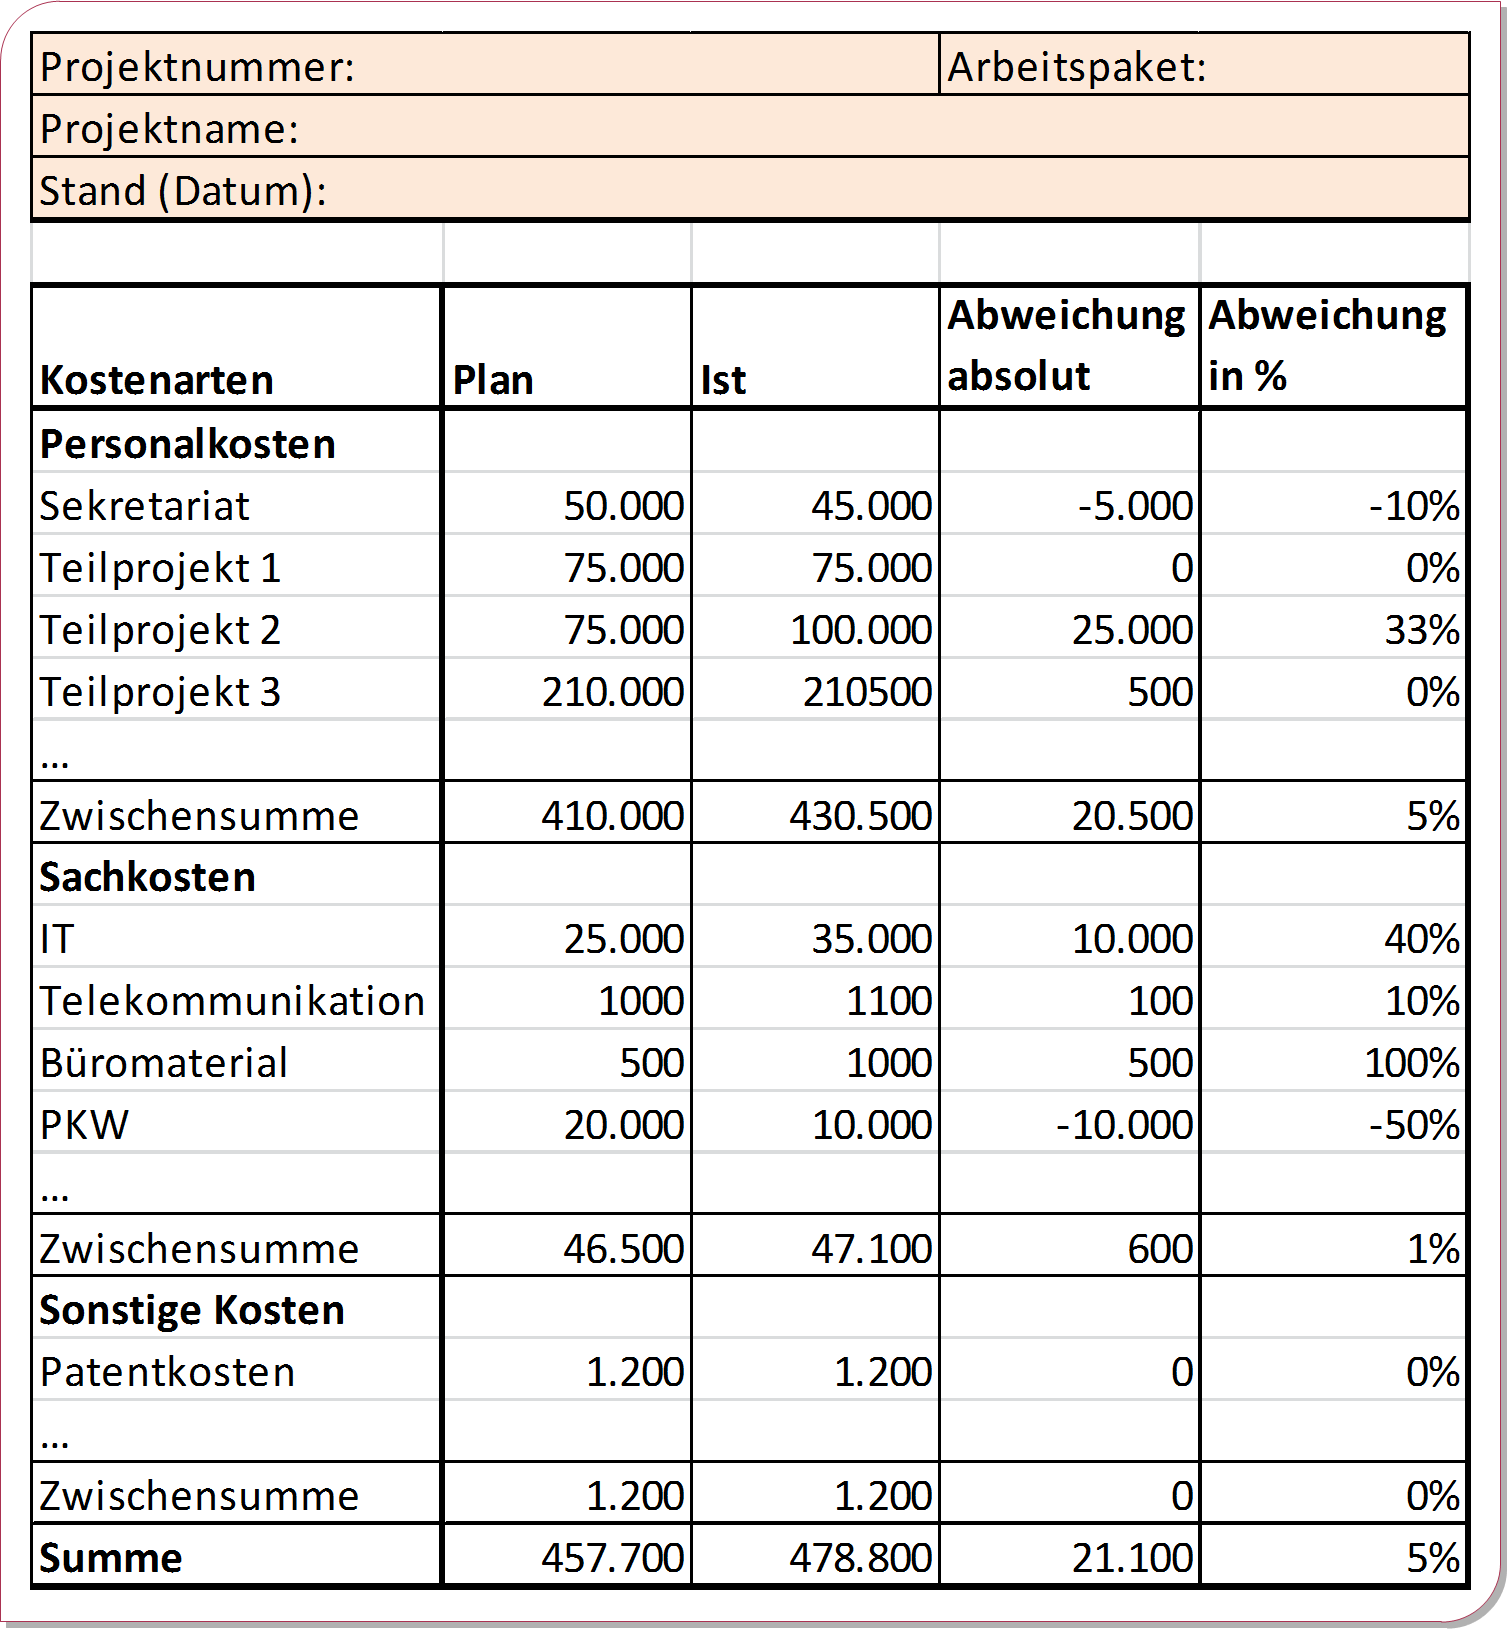
\includegraphics[width=1\textwidth]{Images/PlanIstVergleich.png} 
\begin{center}
   {\footnotesize In Anlehnung an: \cite{Blazek2001}, S. 137}\\
   Einfacher Plan-Ist-Vergleich
   %   \caption[Einfacher Plan-Ist-Vergleich]{Einfacher Plan-Ist-Vergleich}\label{abb3}
\end{center}
%\end{figure}
%\end{floatingfigure}
\newpage
\subsection{Anhang 2}
\label{sec:Anhang2}
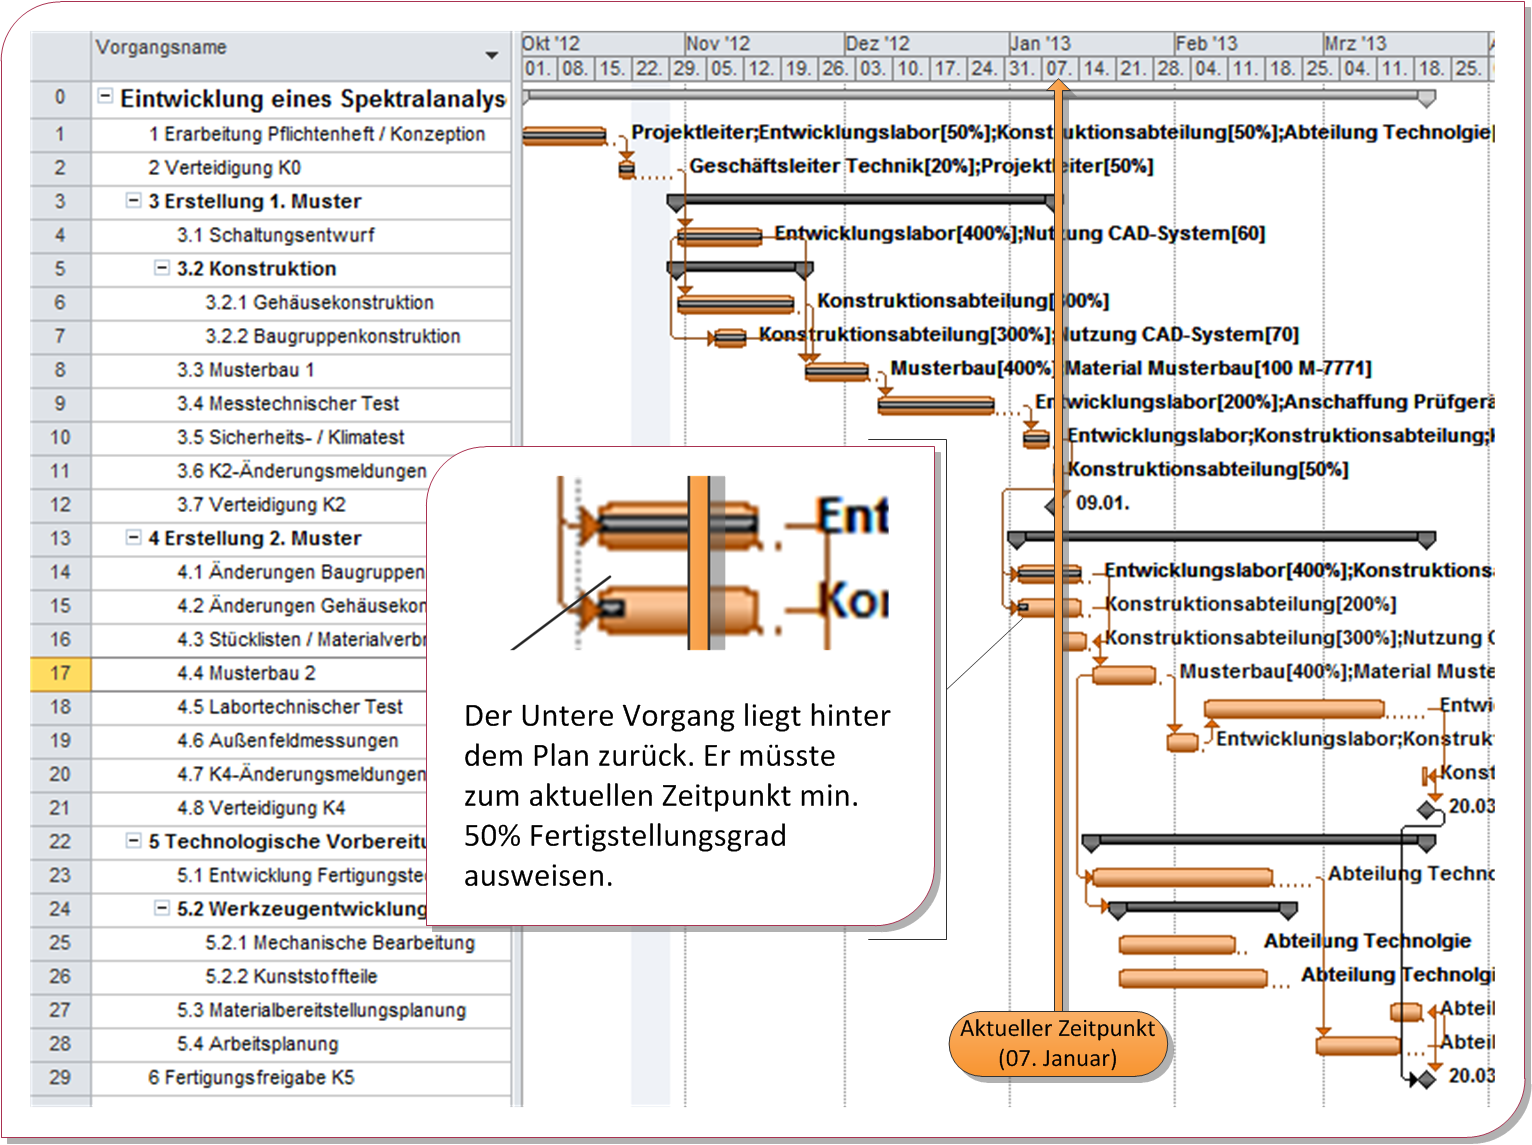
\includegraphics[width=1\textwidth]{Images/MSPfortschritt.png} 
\begin{center}
   %{\footnotesize In Anlehnung an: \cite{Blazek2001}, S. 137}\\
   Projektfortschrittsbericht in MS-Project
   %   \caption[Einfacher Plan-Ist-Vergleich]{Einfacher Plan-Ist-Vergleich}\label{abb3}
\end{center}
%\end{figure}
%\end{floatingfigure}
\newpage
\renewcommand\refname{Literatur- und Quellenverzeichnis}
%\nocite{*}
\bibliographystyle{agsm}
\bibliography{includes/quellen}






\lfoot{\LaTeX}
\end{document}